\documentclass[a4paper, twoside]{article}
\usepackage[utf8]{inputenc} % Especifica la codificación de caracteres de los documentos.
\usepackage[spanish]{babel} % Indica que el documento se escribirá en español.
\usepackage[top=3cm, bottom=2.5cm, inner=1.5cm, outer=2.5cm]{geometry} % Márgenes personalizados
\usepackage{subfiles} % Paquete para incluir el preambulo en los sub archivos.
\usepackage{afterpage} % Permite añadir páginas despues de una página dada.
\usepackage{hyperref} % Permite incluir enlaces en los archivos.
\usepackage{lastpage} % Paquete para poder contabilizar el total de páginas del documento.
\usepackage{fancyhdr} % Permite personalizar los header y footer del documento.
\usepackage{graphicx} % Permite incluir gráficos
\usepackage[hang, bf]{caption} % Personaliza los subtítulos de las figuras y tablas
\usepackage{float} % Permite posicionar mejor las figuras y tablas
\usepackage{amsmath} % Comandos para la escritura de fórmulas matemáticas de mayor complejidad
\usepackage{amsfonts} % Proporciona fuentes matemáticas
\usepackage{amssymb} % Proporciona símbolos matemáticos de la American Mathematical Society
\usepackage{array}
\usepackage{svg}
\usepackage{pgf,tikz}
\usepackage{tikz-timing}
\usepackage{booktabs}

% Defino la ruta de los paquetes personalizados para el apunte
\newcommand{\rutapaquetes}{./paquetes-apunte}

\usepackage[mostrarlicencia]{\rutapaquetes/caratula} % Caratula personalizada (cargada desde caratula.sty)
\usepackage{\rutapaquetes/macros} % Macros útiles para los apuntes (cargado desde macros.sty)
\usepackage[ocultarrevisores]{\rutapaquetes/colaboradores} % Seccion de colaboradores (cargada y creada con colaboradores.sty)
\usepackage{\rutapaquetes/historial} % Seccion de historial de cambios (cargada y creada con historial.sty)

% Define los estilos de los enlaces interpretados por el paquete hyperref
\hypersetup{
	colorlinks=true,   % false: boxed links; true: colored links
	linkcolor=black,   % color of internal links (change box color with linkbordercolor)
	citecolor=green,   % color of links to bibliography
	filecolor=magenta, % color of file links
	urlcolor=blue,     % color of external links
}

\newcommand{\imgdir}{../resources/images} % Ruta de las imágenes

% Define los directorios de las imágenes y gráficos
\graphicspath{ {\imgdir/} {\rutapaquetes/} }

\newcommand{\nombremateria}{Análisis Matemático II (61.03 - 81.01)} % Defino el comando "\nombremateria" para no harcodear el nombre en varios lugares.

% Define el pagestyle personalizado
\pagestyle{fancy}
\fancyhf{}
\renewcommand{\sectionmark}[1]{\markboth{}{\thesection\ \ #1}}
% Define header para pagina par
\fancyhead[ER]{\rightmark}
% Define header para pagina impar
\fancyhead[OL]{\rightmark}
% Define footer para pagina par
\fancyfoot[EL]{\nombremateria \hspace{0.1cm} - Resumen} % Nombre del apunte a la izquierda
\fancyfoot[ER]{Página \thepage\ de \pageref{LastPage}} % Numero de pagina a la derecha
% Define footer para pagina impar
\fancyfoot[OL]{Página \thepage\ de \pageref{LastPage}} % Numero de pagina a la izquierda
\fancyfoot[OR]{\nombremateria \hspace{0.1cm} - Resumen} % Nombre del apunte a la derecha

\renewcommand{\footrulewidth}{0.4pt} % Agrego linea que separa el footer

% Configura la caratula
\materia{\nombremateria}
\tipoapunte{Resumen}
%\tema{Tema de la Materia}
%\subtema{Subtema}

% Defino los entornos de los cuadros
\cuadro{teorema}{blue}
\cuadro{definicion}{gray}
\cuadro{corolario}{green}

\numberwithin{equation}{section}
\numberwithin{figure}{section}
\numberwithin{table}{section}

%\usetikzlibrary{shapes,arrows,positioning,shadows,trees,automata}

\pdfcompresslevel=9

\everymath{\displaystyle}
\newcommand{\vect}[1]{\overline{\textbf{#1}}}
\newcommand{\bayes}{\mathop{\lessgtr}}

\tikzstyle{definicion} = [draw=red, fill=gray!20, very thick,rectangle, rounded corners, inner sep=10pt, inner ysep=20pt]
\tikzstyle{fancytitle} =[fill=red, text=white]

\tikzstyle{corolario} = [draw=red, fill=green!20, very thick,rectangle, rounded corners, inner sep=10pt, inner ysep=20pt]
\tikzstyle{fancytitle} =[fill=red, text=white]

\tikzstyle{teorema} = [draw=red, fill=blue!20, very thick,rectangle, rounded corners, inner sep=10pt, inner ysep=20pt]
\tikzstyle{fancytitle} =[fill=red, text=white]

%------------------------- Inicio del documento ---------------------------

\begin{document}

\maketitle

% Pongo el índice en una página aparte:
\tableofcontents
%\listoffigures
%\listoftables

\subfile{\rutapaquetes/acerca-del-proyecto.tex} % Inlcuye informacion acerca del proyecto FIUBA Apuntes

\section{Introducción al espacio $R^n$}
\subsection{Coordenadas cilíndricas, esféricas y polares}
\begin{table}[H]
	\begin{tabular}{c|c|c}
		\textbf{Cilíndricas} & \textbf{Esféricas} & \textbf{Polares} \\
		\hline
		\parbox{4cm}{
			\begin{center}
				$p \in R^3$, $p=(r,\theta,\bar{z})$ \\
				con $r\geq0,\theta\in[0,2\pi]$
			\end{center}} &
		\parbox{5cm}{
			\begin{center}
				$p\in R^3$, $p=(\rho,\theta,\varphi)$ \\
				con $\rho\geq0,\varphi\in[0,\pi],\theta\in[0,2\pi]$
			\end{center}} &
		\parbox{4cm}{
			\begin{center}
				$p\in R^2,\, p=(r,\theta)$ \\
				con $r\geq0,\theta\in[0,2\pi]$
			\end{center}} \\
		\hline
		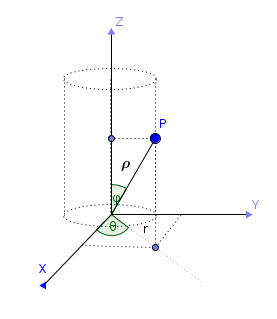
\includegraphics[scale=0.4]{cilindricas} &
		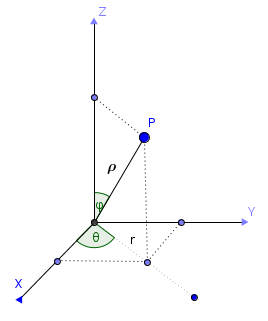
\includegraphics[scale=0.4]{esfericas} &
		\noindent 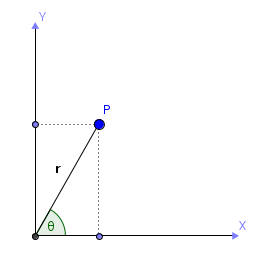
\includegraphics[scale=0.4]{polares} \\
		\hline
		\parbox{5cm}{
			\begin{center}
				$r=c\Rightarrow$ cilindro vertical recto \\
				$\theta=c\Rightarrow$ semiplano vertical \\
				$\bar{z}=c\Rightarrow$ plano horizontal
			\end{center}} &
		\parbox{5cm}{
			\begin{center}
				$r=c\Rightarrow$ esfera concéntrica \\
				$\varphi=c\Rightarrow$ semicono \\
				$\theta=c\Rightarrow$ semiplano
			\end{center}} &
		\parbox{5cm}{
			\begin{center}
				$r=c\Rightarrow$ circunferencia \\
				$\theta=c\Rightarrow$ semirrecta
			\end{center}} \\
		\hline
		\parbox{5cm}{
			\begin{center}
				De cilíndricas a cartesianas:
				$\begin{cases}
				x=r\cdot cos(\theta) \\
				y=r\cdot sin(\theta) \\
				z=\bar{z}
				\end{cases}$ \\
				De cartesianas a cilíndricas:
				$\begin{cases}
				r=\sqrt{x^2+y^2} \\
				\theta=arctan(\frac{y}{x}) \\
				\bar{z}=z
				\end{cases}$
			\end{center}} &
		\parbox{5cm}{
			\begin{center}
				De esféricas a cartesianas:
				$\begin{cases}
				x=\rho\cdot sin(\varphi)cos(\theta) \\
				y=\rho\cdot sin(\varphi)sin(\theta) \\
				z=\rho\cdot cos(\varphi)
				\end{cases}$ \\
				De cartesianas a esféricas:
				$\begin{cases}
				\rho=\sqrt{x^2+y^2+z^2} \\
				\theta=arctan(\frac{y}{x}) \\
				\varphi=arccos(\frac{z}{r})\end{cases}$
			\end{center}} &
		\parbox{5cm}{
			\begin{center}
				De polares a cartesianas:
				$\begin{cases}
				x=r\cdot cos(\theta) \\
				y=r\cdot sin(\theta)
				\end{cases}$ \\
				De cartesianas a polares:
				$\begin{cases}
				r=\sqrt{x^2+y^2} \\
				\theta=arctan(\frac{y}{x})
				\end{cases}$
			\end{center}} \\
	\end{tabular}
\end{table}

\subsection{Secciones cónicas}
\begin{center}
	\setlength{\tabcolsep}{30pt}
	\begin{tabular}{c c}
		\textbf{Circunferencia} & \textbf{Elipse} \\
		$(x-x_0)^2+(y-y_0)^2=r^2$ & $\frac{(x-x_0)^2}{a^2}+\frac{(y-y_0)^2}{b^2}=1$ \\
		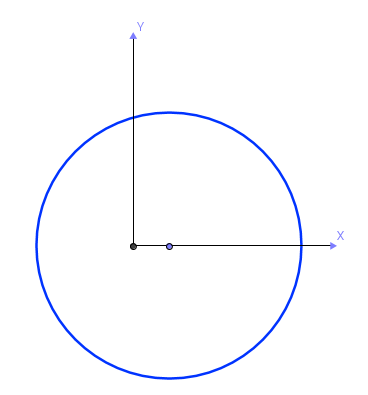
\includegraphics[scale=0.3]{circulo} & 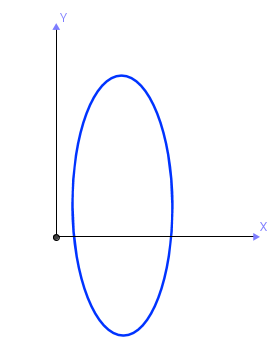
\includegraphics[scale=0.35]{elipse}
	\end{tabular}
	\begin{tabular}{c c}
		\textbf{Parábola} & \textbf{Hipérbola} \\
		$y=ax^2+bx+c$ & $\frac{(x-x_0)^2}{a^2}-\frac{(y-y_0)^2}{b^2}=1$ \\
		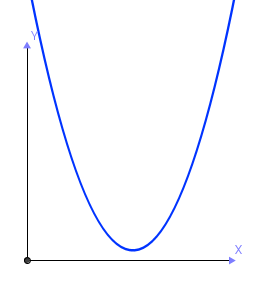
\includegraphics[scale=0.35]{parabola} & 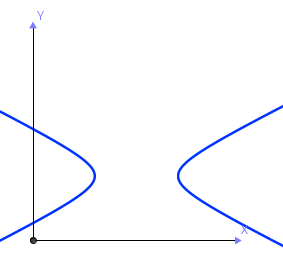
\includegraphics[scale=0.4]{hiperbola}
	\end{tabular}
	\setlength{\tabcolsep}{6pt}
\end{center}

\subsection{Superficies cuádricas}
\begin{center}
	\begin{tabular}{c c c}
		\multicolumn{3}{c}{\textbf{Cilindro}} \\
		\toprule
		Elíptico & Parabólico & Hiperbólico \\
		\parbox{5cm}{
			\begin{center}
				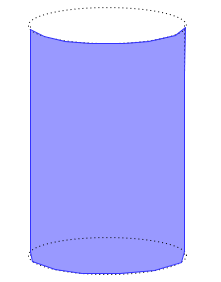
\includegraphics[scale=0.3]{cilindro_eliptico} \\
				$\left(\frac{x}{a}\right)^2+\left(\frac{y}{b}\right)^2=1$
			\end{center}} &
		\parbox{5cm}{
			\begin{center}
				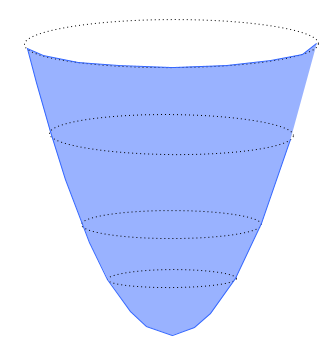
\includegraphics[scale=0.3]{cilindro_parabolico} \\
				$x^2+2rz=0$
			\end{center}} &
		\parbox{5cm}{
			\begin{center}
				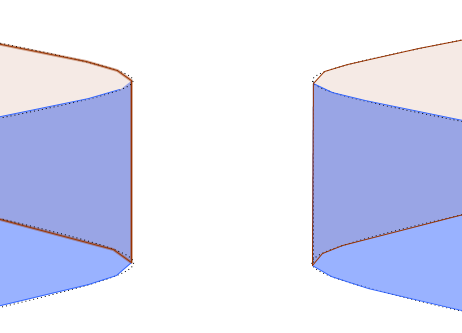
\includegraphics[scale=0.3]{cilindro_hiperbolico} \\
				$\left(\frac{x}{a}\right)^2-\left(\frac{y}{b}\right)^2=1$
			\end{center}} \\
	\end{tabular}

	\begin{tabular}{c | c c}
		\textbf{Cono} & \multicolumn{2}{c}{\textbf{Hiperboloide}} \\
		\hline
		 & De una hoja & De dos hojas \\
		\parbox{5cm}{
			\begin{center}
				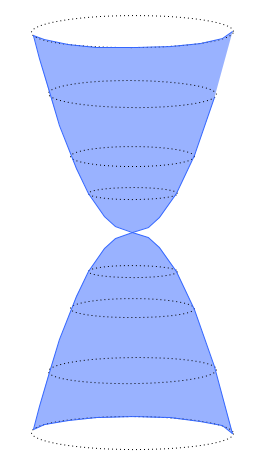
\includegraphics[scale=0.3]{cono} \\
				$\left(\frac{x}{a}\right)^2+\left(\frac{y}{b}\right)^2-\left(\frac{z}{c}\right)^2=0$
			\end{center}} &
		\parbox{5cm}{
			\begin{center}
				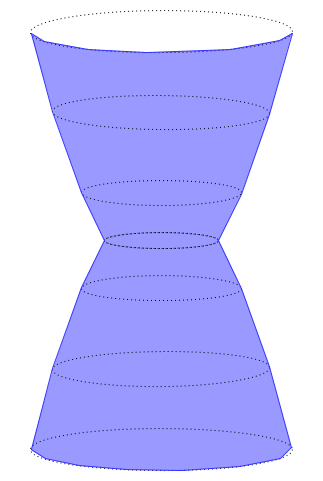
\includegraphics[scale=0.3]{hiperboloide_1hoja} \\
				$\left(\frac{x}{a}\right)^2+\left(\frac{y}{b}\right)^2-\left(\frac{z}{c}\right)^2=1$
			\end{center}} &
		\parbox{5cm}{
			\begin{center}
				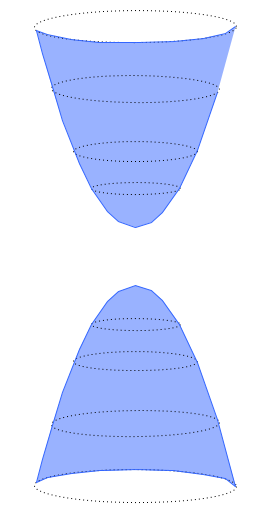
\includegraphics[scale=0.3]{hiperboloide_2hojas} \\
				$\left(\frac{x}{a}\right)^2-\left(\frac{y}{b}\right)^2-\left(\frac{z}{c}\right)^2=1$
			\end{center}} \\
	\end{tabular}

	\begin{tabular}{c | c c}
		\textbf{Elipsoide} & \multicolumn{2}{c}{\textbf{Paraboloide}} \\
		\hline
		 & Elíptico & Hiperbólico \\
		\parbox{5cm}{
			\begin{center}
				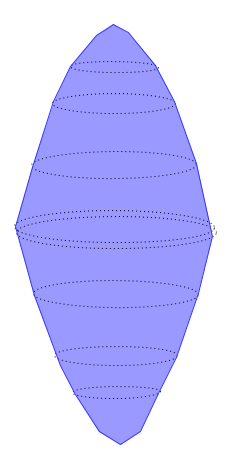
\includegraphics[scale=0.3]{elipsoide} \\
				$\left(\frac{x}{a}\right)^2+\left(\frac{y}{b}\right)^2+\left(\frac{z}{c}\right)^2=1$
			\end{center}} &
		\parbox{5cm}{
			\begin{center}
				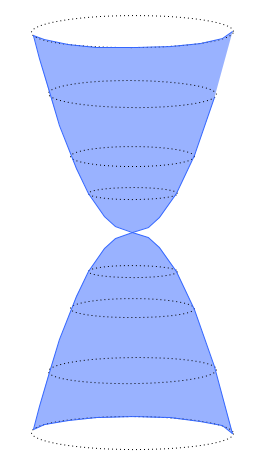
\includegraphics[scale=0.3]{cono} \\
				$z=\left(\frac{x}{a}\right)^2+\left(\frac{y}{b}\right)^2$
			\end{center}} &
		\parbox{5cm}{
			\begin{center}
				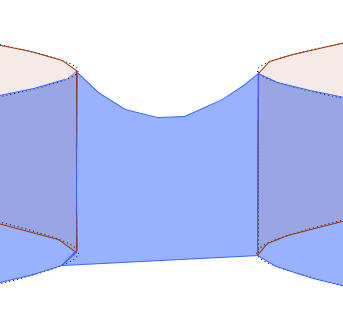
\includegraphics[scale=0.3]{paraboloide_hiperbolico} \\
				$z=\left(\frac{x}{a}\right)^2-\left(\frac{y}{b}\right)^2$
			\end{center}} \\
	\end{tabular}
\end{center}

\subsection{Áreas y volúmenes}
Algunas fórmulas de áreas y volúmenes que conviene recordar:

\begin{center}
	\begin{tabular}{c c c}
		Figura & Superficie & Volumen \\
		\hline
		Elipse & $\pi ab$ & 0 \\
		Circunferencia & $\pi r^2$ & 0 \\
		Esfera & $4\pi r^2$ & $\frac{4}{3}\pi r^3$ \\
		Elipsoide & $4\pi \left(\frac{(ab)^{1.61}+(ac)^{1.61}+(bc)^{1.61}}{3}\right)^\frac{1}{1.61}$ 
		& $\frac{4}{3}\pi abc$ \\
		Cilindro & $2\pi h r$ & $\pi h r^2$ \\
		Cono & $\frac{2}{3}\pi h r$ & $\frac{1}{3}\pi h r^2$ \\
	\end{tabular}
\end{center}

\newpage
\section{Funciones de varias variables}
\subsection{Funciones de varias variables}
\subsubsection{Puntos y conjuntos de puntos en $R^n$}
\begin{enumerate}
	\item \textbf{Entorno de $A\in R^n$}: Un conjunto capaz de incluir una esfera abierta de $R^n$ con centro en $A$ y radio mayor a cero. Se denota como $E(A)$.
	\item \textbf{Entorno reducido de $A\in R^n$}: $E^*(A)=E(A)-\{A\}$
	\item \textbf{Punto aislado}: $A\in S$ es un punto aislado de $S$ cuando existe un $E^*(A)$ que no tiene puntos de $S$.
	\item \textbf{Punto de acumulación}: $A$ es un punto de acumulación de $S$ cuando en todo $E^*(A)$ existe algún punto de $S$.
	\item \textbf{Conjunto abierto}: Aquel que todos sus puntos son interiores.
	\item \textbf{Conjunto cerrado}: Aquel que contiene a todos sus puntos de acumulación.
	\item \textbf{Conjunto acotado}: Aquel que se lo puede incluir en una esfera abierta con radio finito.
	\item \textbf{Conjunto compacto}: Aquel que es cerrado y acotado.
	\item \textbf{Conjunto convexo}: $S$ es convexo cuando $\forall A,B\in S$, el segmento $\overline{AB}$ está incluido en $S$.
	\item \textbf{Conjunto conexo}: $S$ es conexo cuando $\forall A,B\in S$ se puede pasar de $A$ a $B$ desplazándose por $S$.
	\item \textbf{Conjunto simplemente conexo}: $S$ conexo es simplemente conexo cuando toda curva cerrada trazada en él puede, por deformación continua, transformarse en un punto, manteniéndose en el conjunto. En $R^2$, simplemente conexo $\equiv$ conexo sin \emph{agujeros}.
\end{enumerate}

\begin{figure}[H]
	\hspace*{\fill}
	\subfloat[Convexidad]{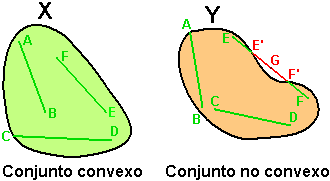
\includegraphics[scale=0.5]{convexidad}}
	\hfill
	\subfloat[A es conexo, B no es conexo]{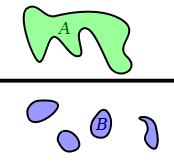
\includegraphics[scale=0.4]{conexidad}}
	\hfill
	\subfloat[El tubo no es simplemente conexo]{\includegraphics[scale=0.3]{\string"simplemente conexo\string".png}}
	\hspace*{\fill}
\end{figure}

\begin{corolario*}{Corolario}
	Dado un conjunto $S\subset R^n$ y un punto $A\in R^n$,pueden ocurrir tres cosas:
	\begin{enumerate}
		\item $A$ es un punto interior a $S$, cuando existe $E(A)$ incluido en $S$,
		\item $A$ es un punto exterior a $S$, cuando existe $E(A)$ que no tiene puntos de $S$,
		\item $A$ es un punto frontera de $S$, cuando para todo $E(A)$ hay puntos en $S$ y puntos que no están en $S$.
	\end{enumerate}
\end{corolario*}

\subsubsection{Función escalar}
\begin{definicion*}{Campo escalar}
	$f:U\subseteq R^n \rightarrow R$. Regla que asocia a cada n-ada ordenada de números reales, (o bien a cada vector $x$ de U), un número real.\\
	
	El conjunto U es el dominio de $f$, su codominio es $R$, y el rango de $f$ es $\{z\in R:\, z=f\left(x\right),\, x\in U\}$.
\end{definicion*}

\subsubsection{Campo vectorial}
\begin{minipage}{0.3\textwidth}
	\begin{figure}[H]
		\centering
		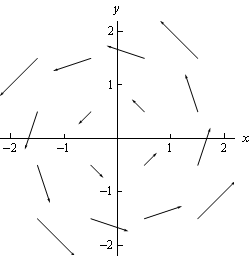
\includegraphics[scale=0.5]{campo_vectorial}
		\caption{Campo vectorial en $R^2$.}
	\end{figure}
\end{minipage}
\begin{minipage}{0.6\textwidth}
	\begin{definicion*}{Campo vectorial}
		$f:U\subseteq R^n \rightarrow R^m$,($m>1)$. Regla que asocia a cada n-ada ordenada de números reales un vector de $R^m$.\\
	\end{definicion*}
\end{minipage}

\subsubsection{Operaciones entre funciones de varias variables}
\begin{definicion*}{Operaciones entre funciones de varias variables}
	Sean $f:U\subseteq R^n \to R$, $g:V\subseteq R^n \to R$, entonces:
	\begin{itemize}
		\item $f + g: U \cap V \subseteq R^n \rightarrow R$ tal que $\left( f + g \right) \left( x \right) = f \left( x \right) + g \left( x \right)$
		\item $f \cdot g: U \cap V \subseteq R^n \rightarrow R$ tal que $\left( fg \right) \left( x \right) = f \left( x \right) \cdot g \left( x \right)$
		\item $\frac{f}{g}: W \subseteq R^n \rightarrow R$ tal que $\left( \frac{f}{g} \right) \left( x \right) = \frac{f \left( x \right)}{g \left( x \right)}$, donde $W = U \cap V - \{x \in V: g \left(x\right) = 0\}$
	\end{itemize}
\end{definicion*}

\subsection{Geometría de las funciones de varias variables}
\begin{definicion*}{Gráfica de $f$}
	Se define la gráfica de $f:U\subseteq R^n \rightarrow R$ al conjunto:
	
	\begin{align}
		\{(x_1,x_2,\ldots,x_n,y)\in R^{n+1}:\overline{x}\in U,y=f(x_1,x_2,\ldots,x_n)\}
	\end{align}
	
	La gráfica de la función $f:U\subseteq R^2 \rightarrow R$ es la gráfica de la superficie $z=f\left(x,y\right)$.\\
	
	Para $n\geq3$,la gráfica no puede ser visualizada. \\
\end{definicion*}

\begin{minipage}{0.6\textwidth}		
	Para graficar, hay que cortar la superficie $z=f(x,y)$ con los planos del tipo $y=kx$ y estudiar el tipo de curvas resultantes.
	En particular, se estudian las curvas resultantes de cortar la superficie con los planos $y=0$ y $x=0$.\\
	
	Otro concepto importante que también se usa como ayuda para obtener gráficos de funciones de dos variables es el de \emph{nivel constante} de una función: dada la función $f:U\subseteq R^n \rightarrow R$ y el número $c\in\mbox{rango de f}$, se define el \emph{\textbf{nivel $c$ de la función $f$}} como el conjunto $N_{c} = \{ x \in U:\, f \left( x \right) = c\}.$\\
	
	Cuando $n=2$, la curva se llama \textit{\textbf{curva de nivel}}. 
	Cuando $n=3$, la curva se llama \textit{\textbf{superficie de nivel}}. 
	El nivel \textit{c}de la superficie $z=f\left(x,y\right)$ se puede interpretar geométricamente como la intersección de la función con el plano $z=c$.
	Estas curvas nos dan idea de la imagen de la función.
\end{minipage}					
\begin{minipage}{0.3\textwidth}
	\begin{figure}[H]
		\centering
		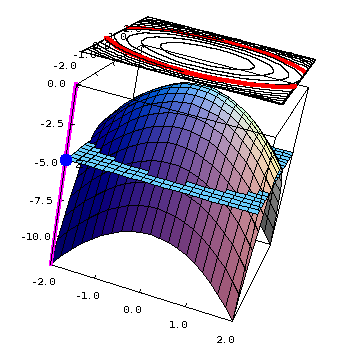
\includegraphics[scale=0.35]{curvas_de_nivel.png}
		\caption{$f(x,y)=-x^2-2y^2$ y sus curvas de nivel.}
	\end{figure}
\end{minipage}

\subsection{Limites y continuidad}
\begin{definicion*}{Bola abierta}
	Sea $x_0\in R^n$ y $r>0$.
	La bola abierta de centro $x_0$ y radio $r$, denotada por $B\left(x_0,r\right)$ es el conjunto de puntos de $R^n$ que distan de $x_0$ en menos que $r$.
\end{definicion*}

\begin{definicion*}{Conjunto abierto}
	Un conjunto $U\subseteq R^n$ es un conjunto abierto de $R^n$ si para cada $x_0\in U$ existe un $r>0$ tal que $B\left(x_0,r\right)\subset U$.
	Esto es, el conjunto $U\subseteq R^n$ será abierto si cuando tomamos un punto $x_0$ en él, este siempre tiene vecinos que siguen viviendo dentro de $U$.\\
\end{definicion*}

\begin{definicion*}{Frontera de un conjunto}
	Sea $U\subseteq R^n$ un subconjunto de $R^n$.
	Un punto $x_0\in R^n$ es un punto frontera de U si toda bola abierta $B(x_0,r)$ contiene puntos en U y fuera de él.
\end{definicion*}

\begin{definicion*}{Límite}
	Sea $f:U\subseteq R^n \rightarrow R$ una función definida en el conjunto abierto U.
	Si $x_0$ es un punto de U o un punto frontera de U, se dice que el límite de $f$ cuando $x$ tiende a $x_0$ es L, lo cual se escribe como $\lim_{x \rightarrow x_0} f \left( x \right) = L$ si dado cualquier $\varepsilon > 0$ existe $\delta > 0$ tal que $x \in B \left( x_{0}, \delta \right) \cap U \left( x \neq x_{0} \right) \Rightarrow f \left( x \right) \in B(L, \varepsilon)$
\end{definicion*}

\begin{definicion*}{Límite por curva}
	Una condición \textit{necesaria} (pero no suficiente) para que el límite $\lim_{ \left( x, y \right) \rightarrow (x_0, y_0) } f \left( x, y \right)$ exista y sea L, es que si los límites $\lim_{ x \rightarrow x_{0} } f \left( x, \phi \left(x \right) \right)$ y $\lim_{ x \rightarrow x_{0} } f \left(x, \psi \left( x \right) \right)$ existen (donde $y = \phi \left( x \right)$ e $y = \psi \left( x \right)$ son curvas que pasan por $\left( x_0, y_0 \right)$) deben valer L. \\

	El único argumento que concluye que un límite existe requiere la aplicación directa de la definición. Para calcular límites también es útil expresar la función en coordenadas polares. \\
	
	\begin{center}
		\textit{Ejemplo}: $\lim_{ \left( x, y \right) \rightarrow (0,0) } \frac{x^{3} y}{x^{2} + y^{2} } = \lim_{ r \rightarrow 0 } \frac{(rcos\theta)^{3} (rsen\theta)}{(rcos\theta)^{2} + (rsen\theta)^{2}} = \lim_{ r \rightarrow 0 } \frac{r^4cos^3(\theta)sen(\theta)}{r^2(\underbrace{ cos^2(\theta) + sen^2(\theta)) }_1} = 0$\\
	\end{center}
\end{definicion*}

\begin{teorema*}{Teorema de límites de funciones}
	Sean $f, g: U \subseteq R^n \rightarrow R$ dos funciones definidas en el abierto U y sea $x_0$ un punto de U o un punto frontera de U.
	Si $\lim_{ x \rightarrow x_0 } f \left( x \right) = L$ y $\lim_{ x \rightarrow x_0 } g \left( x \right) = M$, entonces:
	\begin{align}
		\lim_{x\rightarrow x_{0}}\left(f+g\right)\left(x\right)=L+M \\
		\lim_{x\rightarrow x_{0}}\left(f\cdot g\right)\left(x\right)=L\cdot M \\
		Si M\neq0,\lim_{x\rightarrow x_{0}}\left(\frac{f}{g}\right)\left(x\right)=\frac{L}{M}
	\end{align}
\end{teorema*}

\begin{teorema*}{Continuidad en polinomios}
	Si $f:U\subseteq R^2 \rightarrow R$ es una función polinomial, entonces:
	\begin{align}
		\lim_{\left(x,y\right)\rightarrow(x_0,y_0)}f\left(x,y\right)=f(x_0,y_0)
	\end{align}
\end{teorema*}

\begin{definicion*}{Continuidad en un punto}
	Sea $f: U \subseteq R^n \rightarrow R$ una función definida en el abierto U de $R^n$, y sea $x_0 \in U.$
	Se dice que $f$ es una función continua en $x_{0}$ si $f \left( x_{0} \right) = \lim_{ x \rightarrow x_0} f(x)$.
	Las funciones polinomiales son continuas en cualquier punto $\left( x_0, y_0 \right) \in R^2$.
\end{definicion*}

\begin{definicion*}{Continuidad en un abierto}
	$f: U \subseteq R^n \rightarrow R$ una función definida en el abierto U de $R^n$, se dice continua en $U$ si lo es para todos y cada uno de los puntos $\left(x,y\right)\in U$.
\end{definicion*}

\begin{definicion*}{Continuidad de un campo escalar}
	$f:D\subset R^2 \to R$ es continuo en un punto $\left(x_0,y_0\right)\in D$ si:
	\begin{align} 
		\lim_{(x,y)\to(x_0,y_0)}f(x,y)=f(x_0,y_0)
	\end{align}
\end{definicion*}

\begin{definicion*}{Continuidad y diferenciabilidad de un campo vectorial}
	La función $\vect{f}: U \subseteq R^n \to R^m$, $m>1$, $\vect{f} = \left( f_1, f_2, \ldots, f_m \right)$ es continua en el punto $\vect{x}_0 \in U$ sí y solo si:
	\begin{align}
		f_i:U\subseteq R^n \to R, i=1,2,\ldots,m, \text{ son continuas}
	\end{align}

	La función $\vect{f}: U \subseteq R^n \to R^m$, $m>1$, $\vect{f} = \left( f_1, f_2, \ldots, f_m \right)$ es diferenciable en el punto $\vect{x}_0 \in U$ sí y solo si:
	\begin{align} 
		f_i:U\subseteq R^n \to R, i=1,2,\ldots,m, \text{ son diferenciables}
	\end{align}
\end{definicion*}

\begin{teorema*}{Teorema de continuidad de funciones}
	Sean $f, g: U \subseteq R^n \rightarrow R$ funciones definidas en el abierto $U$ de $R^n$. Si $f$ y $g$ son continuas, entonces:
	\begin{align}
		\text{La función } f+g:U\subseteq R^n \rightarrow R=f\left(x\right)+g(x) \text{ es continua} \\
		\text{La función } f\cdot g:U\subseteq R^n \rightarrow R=f\left(x\right)\cdot g(x) \text{ es continua} \\
		\text{La función } \frac{f}{g}:U\subseteq R^n \rightarrow R=\frac{f\left(x\right)}{g\left(x\right)} \text{ es continua en todo punto } x\in U \text{, donde } g(x)\neq0 \\
		\text{La composición } g\circ f:U\subseteq R^n \rightarrow R \text{ es continua}
	\end{align}
\end{teorema*}

\subsection{Derivadas parciales}
\textbf{Para una función de una variable}: 

\begin{definicion*}{Derivada parcial en $R^1$}
	$f: I \subseteq R \rightarrow R$ definida en el intervalo abierto I, se define la \textit{derivada} de $f$ en $x_0 \in I$:
	\begin{align}
		f^\prime(x_0) = \frac{\partial f}{\partial x}(x_0) = \lim_{h \to 0}\frac{f(x_0+h) - f(x_0)}{h}
	\end{align}
	Si $f^\prime (x_0)$ existe, su valor nos da la pendiente de la recta tangente a la gráfica de la función $y=f(x)$ en el punto $(x_0,y_0)$.
	Para este tipo de funciones, diferenciabilidad equivale a existencia de derivada, y la diferenciabilidad en un punto implica la continuidad de la función en ese punto.
\end{definicion*}

\begin{definicion*}{Derivada parcial en $R^2$}
	$f: U \subseteq R^2 \rightarrow R$ definida en el abierto $U$, con $(x_0, y_0)$ un punto de $U$:
	\begin{align}
		\frac{\partial f}{\partial x}(x_0, y_0) = \lim_{h \to 0}\frac{f(x_0+h, y_0) - f(x_0, y_0)}{h} \\
		\frac{\partial f}{\partial y}(x_0, y_0) = \lim_{h \to 0}\frac{f\left( x_0, y_0 + h \right) - f(x_0, y_0)}{h}
	\end{align}
	Para este tipo de funciones, la existencia de derivadas parciales un punto no implica que la función sea continua en ese punto, por lo que tampoco implica que sea diferenciable en ese punto.
\end{definicion*}

Las derivadas parciales de una función $z = f(x, y)$ en un punto $(x_0, y_0)$ nos hablan del comportamiento geométrico (la inclinación) de las superficie que tal función representa, en las direcciones de los ejes $x$ e $y$.\\

Las derivadas parciales de una función se obtienen \emph{derivando parcialmente} cada una de las variables, y dejando las otras como constantes.\\

\textit{Ejemplo}: sea la función $f(x, y) = 5x^3 + 4xy + y^2$.
Se tiene que $f^\prime_x = 15x^2 + 4y$ y que $f^\prime_y = 4x + 2y$.

\subsection{Derivadas direccionales}
\begin{definicion*}{Derivada direccional}
	Sea $f: U \subseteq R^n \rightarrow R$ una función definida en el conjunto abierto U, y sea $x_0 \in U$. Sea $\vect{v} \in R^n$ un vector \emph{unitario} dado. Se define la derivada de la función $f$ en $x_0$ en la dirección del vector $\vect{v}$:
	\begin{align}
		\frac{\partial f}{\partial \vect{v}} \left( x_0 \right) = \lim_{t \to 0} \frac{f(x_0 + t v_0) - f(x_0)}{t}
	\end{align}
	\begin{align}
		\lim_{h \to 0} \frac{r(h)}{h} = 0
	\end{align}
	El vector unitario $\vect{v}$ se puede escribir como $\vect{v} = (cos(\theta), sin(\theta))$, $0 \leq \theta \leq2 \pi$, entonces:
	\begin{align}
		\frac{\partial f}{\partial \vect{v}}(x_0,y_0) = \lim_{t \to 0} \frac{f(x_0 + tcos(\theta), y_0 + tsin(\theta)) - f(x_0,y_0)}{t}
	\end{align}
	Si $\theta = 0$ se tiene $\frac{\partial f}{\partial v} = \frac{\partial f}{\partial x}$,y si $\theta = \frac{\pi}{2}$ se tiene $\frac{\partial f}{\partial v} = \frac{\partial f}{\partial y}$. 
\end{definicion*}

\subsection{Diferenciabilidad}
\subsubsection{Para funciones de una variable} 
\begin{definicion*}{Diferenciabilidad en $R^1$}
	La función $f: I \subseteq R \rightarrow R$ es \emph{diferenciable} en $x_0 \in I$ si existe una constante $A$ tal que:
	\begin{align}
		f(x_0+h)=f(x_0)+Ah+r(h)
	\end{align}
	\begin{align}
		\lim_{h \to 0}\frac{r(h)}{h}=0
	\end{align}
	El residuo $r(h) \to 0$ más rápidamente que $h$. Despejando A, obtenemos que:
	\begin{align}
		A=\frac{f(x_0+h)-f(x_0)}{h}-\frac{r(h)}{h}
	\end{align}
\end{definicion*}

\subsubsection{Para funciones de dos variable} 
\begin{definicion*}{Diferenciabilidad en $R^2$}
	La función $f:U\subseteq R^2 \rightarrow R$ es \emph{diferenciable} en el punto $(x_0,y_0)$ si hay constantes $A_1$ y $A_2$ tales que:
	\begin{align}
		f((x_0,y_0)+(h_1,h_2))=f(x_0,y_0)+A_1h_1+A_2h_2+r(h_1,h_2)
	\end{align}
	\begin{align}
		\lim_{(h_1,h_2)\rightarrow(0,0)}=\frac{r(h_1,h_2)}{|(h_1,h_2)|}
	\end{align}
	Despejando $A_1$ y $A_2$, obtenemos que:
	\begin{align}
		A_1=\frac{\partial f}{\partial x}(x_0,y_0) \\
		A_2=\frac{\partial f}{\partial y}(x_0,y_0)
	\end{align}
\end{definicion*}

\begin{teorema*}{Teorema diferenciabilidad}
	La función $f: U \subseteq R^2 \rightarrow R$ definida en el abierto $U$ es diferenciable en el punto $(x_0,y_0) \in U$ si:
	\begin{align}
		\exists \text{ } A_1=\frac{\partial f}{\partial x}(x_0,y_0) \\
		\exists \text{ } A_2=\frac{\partial f}{\partial y}(x_0,y_0) \\
		\lim_{(h_1,h_2) \to (0,0)}\frac{r(h_1,h_2)}{|(h_1,h_2)|}=0
	\end{align}
	\begin{align}
		\lim_{(x,y) \to (x_0,y_0)} \frac{f(x,y)-\left[\frac{\partial f}{\partial x}(x_0,y_0)(x-x_0)+\frac{\partial f}{\partial y}(x_0,y_0)(y-y_0)+f(x_0,y_0)\right]}{\sqrt{(x-x_0)^{2}+(y-y_0)^{2}}}=0
	\end{align}
\end{teorema*}

\begin{corolario*}{Corolarios del teorema}
	\begin{itemize}
		\item Si la función es diferenciable en $(x_0,y_0)$, es continua en ese punto.
		\item Las funciones polinomiales $f: R^2 \rightarrow R$ son diferenciables en todo punto.
		\item Si las derivadas parciales son continuas en el punto $\vect{x}_0 \in U$, entonces $f$ es diferenciable en $\vect{x}_0$
	\end{itemize}
\end{corolario*}

\begin{teorema*}{Teorema diferenciabilidad de varias funciones}
	Sean $f,g:U\subseteq R^n \rightarrow R$ dos funciones definidas en $U$, y diferenciables en $(x_0,y_0) \in U.$ Entonces:
	\begin{itemize}
		\item La suma $f+g:U\subseteq R^n \rightarrow R=f(x_0,y_0)+g(x_0,y_0)$	es una función diferenciable en $(x_0,y_0)$.
		\item El producto $f \cdot g:U\subseteq R^n \rightarrow R=f(x_0,y_0)\cdot g(x_0,y_0)$ es una función diferenciable en $(x_0,y_0)$.
		\item Si $g(x_0,y_0) \neq 0$, el cociente $\frac{f}{g}:U\subseteq R^n \rightarrow R=\frac{f(x_0,y_0)}{g(x_0,y_0)}$ es una función diferenciable en $(x_0,y_0)$.
		\item La composición $g \circ f:U\subseteq R^n \rightarrow R$ es diferenciable en $(x_0,y_0)$.
	\end{itemize}
\end{teorema*}

\subsubsection{Para funciones de n variables} 
\begin{definicion*}{Diferenciabilidad  en $R^n$}
	La función $f:U\subseteq R^n \rightarrow R$ es \emph{diferenciable} en el punto $\vect{x}_0$ si hay constantes $A_1,A_2,...,A_n$ tales que:
	\begin{align}
		f(\vect{x}_0+\vect{h})=f(\vect{x}_0)+\sum_{i=1}^{n} A_ih_i+r(\vect{h})
	\end{align}
	\begin{align}
		\lim_{\vect{h} \to \vect{0}}=\frac{r(\vect{h})}{|\vect{h}|}
	\end{align}
	Despejando $A_1$ y $A_2$, obtenemos que:
	\begin{align}
		A_i=\frac{\partial f}{\partial x_i}(\vect{x}_0), \forall i=1,...,n
	\end{align}
\end{definicion*}

\begin{teorema*}{Teorema de la diferenciabilidad y las derivadas direccionales}
	Sea $f:U\subseteq R^n \rightarrow R$ \textit{\emph{diferenciable}}, definida en el conjunto abierto U. Sea $x_0\in U$ y sea $\vect{v}\in R^n$ el vector unitario en cuya dirección queremos calcular la derivada de la función $f$ en el punto $x_0.$ Entonces:
	\begin{align}
		\frac{\partial f}{\partial\vect{v}}(x_{0})=\sum_{i=1}^{n}\frac{\partial f}{\partial x_{i}}(x_0)\cdot\vect{v}_{i}
	\end{align}
	\textit{Ejemplo}: dada $f:R^2 \rightarrow R$ tal que $f(x,y)=x^2+y^2,$ queremos calcular la derivada de la función en un punto arbitrario $(x_{0},y_{0})\in R^2$ en la dirección del vector unitario $\vect{v}=(cos(\theta),sin(\theta))$.\\

	Dado que la función es polinomial, es diferenciable en todo el dominio.\\

	Entonces según la fórmula se tiene que:\\
	\begin{align}
		\frac{\partial f}{\partial v}(x_0,y_0)=\frac{\partial f}{\partial x}(x_0,y_0)cos(\theta)+\frac{\partial f}{\partial y}(x_0,y_0)sen(\theta)=2x_0cos(\theta)+2y_0sen(\theta)
	\end{align}
\end{teorema*}

\subsection{Gradiente}
\begin{minipage}{0.31\textwidth}
	\begin{figure}[H]
		\centering
		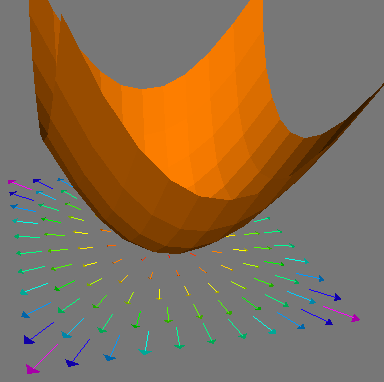
\includegraphics[scale=0.23]{campo_de_gradientes.png}
		\caption{El gradiente apunta a la dirección de mayor variación.}
	\end{figure}
\end{minipage}
\begin{minipage}{0.6\textwidth}
	\begin{definicion*}{Gradiente de una función}
		Sea $f:U\subseteq R^n \rightarrow R$ una función diferenciable definida en el conjunto abierto U de $R^n$.Se define el vector gradiente de la función $f$ en el punto $x_0\in U$ como el vector de $R^n$ dado por: \\
		\begin{align}
			\nabla f(x_0)=(f^\prime_{x_1}(x_0),f^\prime_{x_2}(x_0),\ldots,f^\prime_{x_n}(x_0))
		\end{align}
		\begin{align}
			\nabla f(x_0)\cdot\vect{v}=f^\prime_{\vect{v}}(x_0)
		\end{align}
		
		El vector $\nabla f(x_0)$ nos dice en qué dirección se tiene la mayor variación (el mayor crecimiento) de la función $f$ en el punto	$x_0$.\\
		
		Además, se tiene que el vector $\nabla f(x_0)$ es un vector ortogonal a la curva de nivel que pasa por $x_0$.
	\end{definicion*}
\end{minipage}

\begin{corolario*}{Propiedades del gradiente}
	Si $f$ es diferenciable, la dirección de la derivada direccional	puede ser
	\begin{itemize}
		\item Máxima: $v=\frac{\nabla f}{\left|\nabla f\right|}$, y su valor es $\left|\nabla f\right|$
		\item Mínima: $v=-\frac{\nabla f}{\left|\nabla f\right|}$, y su valor es $-\left|\nabla f\right|$
		\item Nula: $v\bot\nabla f$, y su valor es 0
	\end{itemize}
\end{corolario*}

\subsection{Vectores normales}
\begin{definicion*}{Vectores normales}
	Dada una función diferenciable $f:U\subseteq R^2 \rightarrow R$ definida en el conjunto abierto U de $R^2$ tal que $z=f(x,y)$, y dado un punto $p=(x_0,y_0,f(x_0,y_0))$, el vector normal $N_{p}$ a la superficie de la función en el punto $(x_0,y_0)$ se obtiene mediante:
	\begin{align}
		\vect{N}_{p}=\left|\begin{array}{ccc}
		\hat{i} & \hat{j} & \hat{k}\\
		\frac{\partial f_x}{\partial x} & \frac{\partial f_y}{\partial x} & \frac{\partial f_z}{\partial x}\\
		\frac{\partial f_x}{\partial y} & \frac{\partial f_y}{\partial y} & \frac{\partial f_z}{\partial y}\end{array}\right|_{p}=\left|\begin{array}{ccc}
		\hat{i} & \hat{j} & \hat{k}\\
		1 & 0 & f^\prime_{x}(x_0,y_0)\\
		0 & 1 & f^\prime_{y}(x_0,y_0)\end{array}\right|=(-f^\prime_{x}(x_0,y_0),-f^\prime_{y}(x_0,y_0),1)
	\end{align}
\end{definicion*}

\underbar{Nota}: recordar que la superficie $z=f(x,y)$ se puede ver  como el nivel 0 de la función $F(x,y,z)=z-f(x,y)$. De allí el porqué de la última coordenada del vector. Suele presentarse como $(f^\prime_{x}(x_0,y_0),f^\prime_{y}(x_0,y_0),-1)$ que luego es \underline{mal llamado gradiente extendido}.

\subsection{Planos tangentes y rectas normales}
\begin{definicion*}{Plano tangente}
	Si la función $f:U\subseteq R^2 \rightarrow R$ es diferenciable en el punto $(x_0,y_0)$, entonces la siguiente ecuación define al \textbf{plano tangente} a la superficie $z=f(x,y)$ en el punto $(x_0,y_0,f(x_0,y_0))$:
	\begin{align}
		z=f(x_0,y_0)+f^\prime_{x}(x_0,y_0)(x-x_0)+f^\prime_{y}(x_0,y_0)(y-y_0)
	\end{align}
	De la ecuación anterior se deduce que el plano tangente en un punto $(x_0,y_0)$ es un plano que pasa por el punto y contiene a las rectas tangentes en el punto.\\
	Es decir, tiene como vector normal al vector $\vect{N}_{(x_0,y_0)}=(\nabla f(x_0,y_0),-1)$ calculado anteriormente.
\end{definicion*}

\begin{minipage}{0.25\textwidth}
	\begin{figure}[H]
		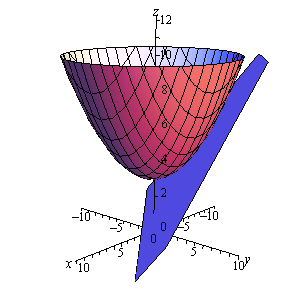
\includegraphics[scale=0.3]{plano_tangente.png}
		\caption{Plano tangente}
	\end{figure}
\end{minipage}
\begin{minipage}{0.8\textwidth}
	\begin{definicion*}{Recta normal}
		Dada una función diferenciable $f:U\subseteq R^2 \rightarrow R$ cuya gráfica es una superficie $S$, se define la \textbf{recta normal} a la superficie $S$ en el punto $p=(x_0,y_0,z_0)$ de ella, como la recta que pasa por $p$ y contiene al vector normal a la superficie en $p.$ Su ecuación está dada por:
		\begin{align}
			L:\:(x,y,z)=t(f^\prime_{x}(x_0,y_0),f^\prime_{y}(x_0,y_0),-1)+(x_0,y_0,z_0), \text{ } t \in R
		\end{align}
	\end{definicion*}
\end{minipage}

\subsection{Diferencial}
\begin{definicion*}{Diferencial}
	Dada la función $f:U\subseteq R^n \rightarrow R$ diferenciable, la diferencial de $f$ se define como:
	\begin{align}
		df=\sum_{i=1}^{n}\frac{\partial f}{\partial x_i}\partial x_i
	\end{align}
	\textit{Ejemplo}: el diferencial de $f(x)=sen^3(x^2)$	es:
	\begin{align}
		df=3sen^2(x^2)cos(x^2)2xdx=6xsen^2(x^2)cos(x^2)dx
	\end{align}
\end{definicion*}

\subsection{Derivadas parciales de órdenes superiores}
Dada una función $f: U \subset R^2 \rightarrow R$ definida en el conjunto abierto $U$ de $R^2$. Si la función es diferenciable, entonces existen las derivadas parciales $\frac{\partial f}{\partial x}$ y $\frac{\partial f}{\partial y}$ en cualquier punto $(x,y)\in U$.\\

Puede ocurrir que estas derivadas sean lo suficientemente \emph{bien portadas} en $U$ como para que podamos obtener de ellas sus derivadas parciales $\frac{\partial}{\partial x}\left(\frac{\partial f}{\partial x}\right),\frac{\partial}{\partial y}\left(\frac{\partial f}{\partial x}\right),\frac{\partial}{\partial x}\left(\frac{\partial f}{\partial y}\right),\frac{\partial}{\partial y}\left(\frac{\partial f}{\partial y}\right)$.\\

\begin{teorema*}{Teorema de Schwarz}
	Sea $f:U\subseteq R^2 \rightarrow R$ una función definida en el abierto $U$ de $R^2$. Si:
	\begin{align}
		\exists \frac{\partial^2 f}{\partial x\partial y}:U\subseteq R^2 \rightarrow R \\
		\exists \frac{\partial^2 f}{\partial y\partial x}:U\subseteq R^2 \rightarrow R
	\end{align}
	Y son funciones continuas en $U$, entonces:
	\begin{align}
		 \frac{\partial^2 f}{\partial x\partial y}=\frac{\partial^2 f}{\partial y\partial x}
	\end{align}
\end{teorema*}

\subsection{Funciones de clase $\mathcal{C}^{\mathbf{k}}$}
\begin{definicion*}{Funciones de clase $\mathcal{C}^k$}
	$f$ es una función $k$ veces diferenciable si la función $f^{(k-1)}:I\subseteq R \rightarrow R$ es diferenciable.\\
	
	Si $f$ es $k$ veces diferenciable para todo $k\in N$, se dice ser infinitamente diferenciable, o bien, de clase $\mathcal{C}^{\infty}$.\\
	
	En particular, sea $f:I\subseteq R \rightarrow R$ una función diferenciable. Si la función derivada $f^\prime$ es continua, se dice que $f$ es una función de clase $\mathcal{C}^{1}$. Si esta función $f^\prime$ es, a su vez, una función diferenciable, decimos que $f$ es una función dos veces diferenciable.
\end{definicion*}

\begin{corolario*}{Corolario}
	Si la función $f: U \subseteq R^n \rightarrow R$ es de clase $\mathcal{C}^{1}$, entonces $f$ es diferenciable.
\end{corolario*}

\newpage
\section{Funciones compuestas, inversas e implícitas}
\subsection{Composición de funciones}
\begin{definicion*}{Composición de funciones}
	Si tenemos las funciones $g: I \subseteq R \rightarrow R$ y $f: J \subseteq R \rightarrow R$ (tales que $g(I) \subseteq J$), podemos formar la composición $f\circ g:I\subseteq R \rightarrow R$.\\
			
	Si $g:I\subseteq R \rightarrow R$ es diferenciable en un punto $x_0 \in I$ y $f:J\subseteq R \rightarrow R$ es diferenciable en $g(x_0)\in J$, entonces la composición $f\circ g$ es diferenciable en $x_0$, es decir, que $(f\circ g)^\prime(x)$ existe, y $(f\circ g)^\prime(x)=f^{\prime}(g(x))g^{\prime}(x)$.
\end{definicion*}

\begin{definicion*}{Composicion de funciones de $R^2$}
	Para el caso de dos variables, tenemos que $z=f(x,y)$. Para \emph{componer} esta función tendremos que sustituir las \textit{dos variables} ($x$ e $y$) por \textit{dos funciones}, $g_1$ y $g_2$, que conecten a éstas con \textit{otras} variables,  $u$ y $v$.\\
	
	Si consideramos las funciones $x=g_1(u,v)$ e $y=g_2(u,v)$, podemos sustituir éstas en la función $f$ y obtener la \textbf{función compuesta} :
	\begin{align}
		y=f(g_1(u,v),g_2(u,v))
	\end{align}
\end{definicion*}

\begin{definicion*}{Composicion de funciones de $R^n$}
	Si tenemos la función $f: U \subseteq R^n \rightarrow R$ definida en el conjunto $U$, y la función $g: V \subseteq R^n \rightarrow R$ definida en el conjunto $V$, cuyo rango está contenido en $U$ (i.e. tal que $g(V) \subseteq U$) entonces podemos formar la composición $f\circ g:V\subseteq R^n \rightarrow R$, como:
	\begin{align}
		(f\circ g)(\vect{v})=f(g(\vect{v})),v\in V.
	\end{align}
\end{definicion*}

\subsection{Regla de la cadena}
\begin{teorema*}{Regla de la cadena}
	Sea $g: V \subseteq R^m \to R^n$ una función definida en el conjunto abierto V de $R^m$, diferenciable en $x_0 \in V$. Sea $f:U\subseteq R^n \to R$ una función definida en el conjunto abierto U de $R^n$, tal que $g(V) \subseteq U$, diferenciable en el punto $g(x_0) \in U$:
	\begin{align}
		f\circ g:V\subseteq R^m \to R \text{ es diferenciable en } x_0 \\
		\frac{\partial}{\partial x_j}(f \circ g)(x_0) = \sum_{i=1}^{n}\frac{\partial f}{\partial y_i}(g(x_0)) \frac{\partial g_i}{\partial x_j} (x_0) \text{ , } j=1,2,\ldots,m
	\end{align}
\end{teorema*}

\subsection{Regla de la cadena: perspectiva general}
\begin{definicion*}{Regla de la cadena general}
	Sea la función $f:U\subseteq R^n \to R^m$ definida en el conjunto abierto U de $R^n$, y sea $x_0\in U$.\\
			
	Se dice que esta función es diferenciable en $x_0$ si existe una transformación lineal $f^\prime (x_0):R^n \to R^m$, llamada derivada de $f$ en $x_0$ tal que:
	
	\begin{align}
		f(x_0+h)=f(x_0)+f^\prime(x_0)h+r(h) \text{ ,donde } \lim_{h\to0}\frac{r\left(h\right)}{\left|\left|h\right|\right|}=0
	\end{align}
	(para $h \in R^n$ tal que $x_0+h\in U$).\\
	
	La matriz de esta transformación $f^\prime(x_0) R^n\to R^m$ es:
	\begin{align}							 
		\left[\begin{array}{ccc}
		\frac{\partial f_1}{\partial x_1}(x_0) & \cdots & \frac{\partial f_1}{\partial x_n}(x_0)\\
		\vdots & \ddots & \vdots\\
		\frac{\partial f_m}{\partial x_1}(x_0) & \cdots & \frac{\partial f_m}{\partial x_n}(x_0)\end{array}\right]
	\end{align}
	
	Esta matriz de $m\times n$ se llama \textbf{matriz jacobiana} de la función $f$ en $x_0$ y se denota $Jf(x_0)$. Esta es, entonces, la derivada de la función diferenciable $f$ en $x_0$. En el caso de que $m=1$, la matriz jacobiana se identifica de manera natural con el vector gradiente de $f$ en $x_0$.\\
\end{definicion*}

\textit{Ejemplo}: sea $f: R^2 \to R^3$ dada por $f(x,y)=(\overbrace{sen\left(x+y\right)}^{f_1},\overbrace{xe^{x+y}}^{f_2},\overbrace{x+y}^{f_3})$.\\

$f$ es diferenciable en todo su dominio, y su derivada en el punto	$(0,0)$ está dada por la matriz:\\

$Jf(0,0)=\left[
	\begin{array}{cc}
		\frac{\partial f_{1}}{x}\left(0,0\right) & \frac{\partial f_{1}}{y}\left(0,0\right)\\
		\frac{\partial f_{2}}{x}\left(0,0\right) & \frac{\partial f_{2}}{y}\left(0,0\right)\\
		\frac{\partial f_{3}}{x}\left(0,0\right) & \frac{\partial f_{3}}{y}\left(0,0\right)
	\end{array}\right]=\left[
	\begin{array}{cc}
		cos\left(x+y\right) & cos\left(x+y\right)\\
		e^{x+y}\left(x+1\right) & xe^{x+y}\\
		1 & 1
	\end{array}\right]_{(0,0)}=\left[
	\begin{array}{cc}
		1 & 1\\
		1 & 0\\
		1 & 1
	\end{array}\right]$

\vspace{0.5cm}

\begin{teorema*}{Regla de la cadena en funciones compuestas}
	Sea $f:U\subseteq R^n \to R^p$ una función definida en el abierto $U$ de $R^n$, y $g:V\subseteq R^m \to R^n$ una función definida en el abierto V de $R^m$ tal que $g(V)\subseteq U.$ Si $g$ es diferenciable en $x_0\in V$ y $f$ es diferenciable en $g(x_0)\in U$, entonces la función $f\circ g:V\subseteq R^m \to R^p$ es diferenciable en $x_0$ y su derivada viene dada por la matriz:
	\begin{align}
		J(f\circ g)(x_0)=Jf(g(x_0))\cdot Jg(x_0)
	\end{align}
\end{teorema*}

\subsection{Funciones Implícitas (I)}
\begin{teorema*}{Teorema de la función implícita (1\textsuperscript{ra} versión)}
	Sea $z=F(x,y)$, y sea $(x_0,y_0) \in R^2$ un punto. Si:
	\begin{enumerate}
		\item $F\left(x_{0},y_{0}\right)=0$
		\item La función F tiene derivadas parciales continuas en un entorno de $(x_0,y_0)$
		\item $\frac{\partial F}{\partial y}(x_0,y_0)\ne0$
	\end{enumerate}
	Entonces $F(x,y)=0$ se puede resolver para $y$ en términos de $x$ y definir así una función $y=f(x)$ con dominio en una vecindad de $x_0$, tal que $y_0=f(x_0)$, la cual tiene derivadas continuas en $V$ que pueden calcularse como:
	\begin{align}
		y^{'}=f^{'}\left(x\right)=-\frac{\frac{\partial F}{\partial x}(x,y)}{\frac{\partial F}{\partial y}(x,y)} \text{ , } x\in V.
	\end{align}
	\underbar{Nota 1}: Este teorema es de \textit{existencia}, es decir, nos puede decir si existe una función $y=f(x)$ definida implícitamente por $F(x,y)=0$, pero \textit{no} nos dice cómo se determina tal función.\\
	
	\underbar{Nota 2}: Este teorema es \textit{local}. Nos asegura la existencia de la función $y=f(x)$, o nos asegura la posibilidad del despeje de $y$ en términos de $x$ a partir de $F(x,y)=0$ \textit{solamente en las cercanías del punto }$(x_0,y_0)$. Fuera de la vecindad $V$, el teorema no se responsabiliza por la existencia de la función $f$.
\end{teorema*}

\begin{corolario*}{Recta tangente de funciones implícitas}
	La ecuación de la recta tangente a la curva $F(x,y)=0$ en $(x_{0},y_{0})$ está dada por
	\begin{align}
		\frac{\partial F}{\partial x}(x_0,y_0)(x-x_0)+\frac{\partial F}{\partial y}(x_0,y_0)(y-y_0)=0
	\end{align}
\end{corolario*}

\begin{corolario*}{Recta normal de funciones implícitas}
	La ecuación de la recta normal a la curva $F(x,y)=0$ en $(x_{0},y_{0})$ está dada por
	\begin{align}
		\frac{\partial F}{\partial x}(x_0,y_0)(x-x_0)-\frac{\partial F}{\partial y}(x_0,y_0)(y-y_0)=0
	\end{align}
	Muy similar a la recta tangente, ¿Qué sutil puede ser un signo, no?
\end{corolario*}

\begin{teorema*}{Teorema de la función implícita (2\textsuperscript{da} versión)}
	Sea la función $z=F(x_1,x_2,\ldots,x_n,y)$ y sea $p=(\overline{x_1},\overline{x_2},\ldots,\overline{x_n},\overline{y}) \in R^{n+1}$ un punto tal que $F\left(p\right)=0$.\\
	
	Suponemos que la función $F$ tiene derivadas parciales $\frac{\partial F}{\partial x_i},i=1,2,\ldots,n$ y $\frac{\partial F}{\partial y}$ continuas en alguna bola $B$ con centro en $p$ y que $\frac{\partial F}{\partial y}(p)\ne0$.\\
	
	Entonces $F(x_1,x_2,\ldots,x_n,y)=0$ puede resolverse para $y$ en términos de $x$ y definir así una vecindad $V$ (de $R^n$) del punto $(\overline{x_1},\overline{x_2},\ldots,\overline{x_n},\overline{y})$,una función $y=f(x_1,x_2,\ldots,x_n)$ la cual tiene derivadas parciales continuas en $V$ que se pueden calcular con las fórmulas:
	\begin{align}
		\frac{\partial f}{\partial x_i}(x_1,x_2,\ldots,x_n)=\frac{\frac{\partial F}{\partial x_i}(x_1,x_2,\ldots,x_n,y)}{\frac{\partial F}{\partial y}(x_1,x_2,\ldots,x_n,y)} \text{ con } (x_1,x_2,\ldots,x_n) \in V
	\end{align}
\end{teorema*}

\begin{teorema*}{Teorema de la función implícita (3\textsuperscript{ra} versión)}
	Sean $z_1=F(x,y,u,v)$ y $z_2=G(x,y,u,v)$. Sea $p=(x_0,y_0,u_0,v_0) \in R^4$ un punto tal que $F(p)=G(p)=0$, las funciones $F$ y $G$ tienen todas sus derivadas parciales continuas en un entorno de $p$, y que $\frac{\partial(F,G)}{\partial(u,v)}(p)\ne0$.\\
			
	Entonces $z_1$ y $z_2$ definen funciones implícitas $u=\varphi_1(x,y)$ y $v=\varphi_2(x,y)$, definidas en una una vecindad $V$ de $(x_0,y_0)$, las cuales tienen derivadas parciales continuas en $V$ que se pueden calcular con las fórmulas:
	\begin{align}
		\frac{\partial u}{\partial x}=-\frac{\frac{\partial(F,G)}{\partial(x,v)}}{\frac{\partial(F,G)}{\partial(u,v)}},\frac{\partial u}{\partial y}=-\frac{\frac{\partial(F,G)}{\partial(y,v)}}{\frac{\partial(F,G)}{\partial(u,v)}},\frac{\partial v}{\partial x}=-\frac{\frac{\partial(F,G)}{\partial(u,x)}}{\frac{\partial(F,G)}{\partial(u,v)}},\frac{\partial v}{\partial y}=-\frac{\frac{\partial(F,G)}{\partial(u,y)}}{\frac{\partial(F,G)}{\partial(u,v)}}
	\end{align}
	\underline{Notación:} si $X$ e $Y$ son funciones de las variables $x$ e $y$, se llama \textbf{jacobiano} de $X$ e $Y$ respecto de $x$ e $y$, denotado por $J\left(\frac{X,Y}{x,y}\right)=\frac{\partial\left(X,Y\right)}{\partial\left(x,y\right)}$ al determinante $\frac{\partial\left(X,Y\right)}{\partial\left(x,y\right)}=\left|\begin{array}{cc}\frac{\partial X}{\partial x} & \frac{\partial X}{\partial y}\\
	\frac{\partial Y}{\partial x} & \frac{\partial Y}{\partial y}\end{array}\right|$
\end{teorema*}

\begin{teorema*}{Teorema de la función implícita (4ta versión)}
	Considere las $n$ funciones $u_i=F_i(x_1,\ldots,x_m,y_1,\ldots,y_n)$ con $i=1,2,\ldots,n$.\\
	
	Sea $p=(\overline{x_1},\ldots,\overline{x_m},\overline{y_1},\ldots,\overline{y_m}) \in R^{m+n}$ un punto tal que $F_i(p)=0$ con $i=1,2,\ldots,n$.\\
	
	Suponga que $F_i$ tiene sus $m+n$ derivadas parciales continuas en un entorno de $p$.\\
	
	Si el jacobiano $\frac{\partial(F_1,F_2,\ldots,F_n)}{\partial(y_1,y_2,\ldots,y_n)}(p)\ne0$, entonces las expresiones $F_i(x_1,\ldots,x_m,y_1,\ldots,y_n)$ definen funciones implícitas $y_i=\varphi_i(x_1,\ldots,x_m)$ con $i=1,2,\ldots,n$ definidas en una vecindad $V$ de ($\overline{x_1},\ldots,\overline{x_m})$, las cuales tienen derivadas parciales continuas en $V$ que se pueden calcular como:
	\begin{align}
		\frac{\partial y_i}{\partial x_j}=-\frac{\frac{\partial(F_1,F_2,\ldots,F_n)}{\partial(y_1,\ldots,y_{i-1},x_j,y_{i+1},\ldots,y_n)}}{\frac{\partial(F_1,F_2,\ldots,F_n)}{\partial(y_1,y_2,\ldots,y_n)}}
	\end{align}
\end{teorema*}

\begin{definicion*}{Curvas como intersección de superficies}
	Dado el sistema de ecuaciones $\left\{ \begin{array}{c} F\left(x,y,z\right)=0 \\ G\left(x,y,z\right)=0\end{array}\right.$ y el punto $A=(x_0,y_0,z_0)$. Cuando:
	\begin{enumerate}
		\item $F(A)=0$ y $G(A)=0$,
		\item $\nabla F,\nabla G\in C^{1}(E(A)),$
		\item $\nabla F(A)\neq0$ y $\nabla G(A)\ne0$,
	\end{enumerate}
	El sistema define una curva $\mathcal{C}$ que pasa por $A$, y que admite recta tangente y plano normal en $A$, siendo $d_0=\nabla F(A)\times\nabla G(A)$ el vector director de la recta tangente.
\end{definicion*}

\begin{definicion*}{Superficies definidas en forma implícita}
	Sea $F(x,y,z)=0$ con $F$ escalar y un punto $A=(x_0,y_0,z_0)$, tal que:
	\begin{enumerate}
		\item $F(A)=0$
		\item $\nabla F$ es $\mathcal{C}^{1}$ en $E(A),$
		\item $\nabla F(A)\ne0,$
	\end{enumerate}
	Entonces $F(x,y,z)=0$ es la ecuación de una superficie que pasa por $A$ y admite recta normal y plano tangente en $A$. Además, se tiene que si $\frac{\partial F}{\partial z}(A)\ne0$, entonces $F(x,y,z)=0$ define a $z=f(x,y)$ en un entorno de $A$.
\end{definicion*}

\subsection{Funciones inversas}
\begin{definicion*}{Funciones inversas}
	Si $F:U\subseteq R^2 \to R$ es una función tal que $F(\overline{u},\overline{v})=(\overline{x},\overline{y})$ y en un entorno de $(\overline{u},\overline{v})$ las derivadas parciales $\frac{\partial f}{\partial u},\frac{\partial f}{\partial v},\frac{\partial g}{\partial u},\frac{\partial g}{\partial v}$ de las funciones coordenadas de $F$ son continuas (i.e. $F$ es de clase $\mathcal{C}^{1})$, se tiene que siendo el determinante de $JF(\overline{u},\overline{v})\ne0$, entonces existe un entorno de $(\overline{x},\overline{y})$ en la que existe la inversa $F^{-1}$ de la función $F$, la cual tiene continuas las derivadas parciales de sus funciones coordenadas en el entorno, y su matriz jacobiana es $JF^{-1}(x,y)=\left(JF(u,v)\right)^{-1}$ donde $(x,y)=(f(u,v),g(u,v)) \in E((\overline{x},\overline{y}))$:
	\begin{align}
		(F^{-1})'(x,y)=\left(F'(u,v)\right)^{-1}
	\end{align}
\end{definicion*}

\begin{teorema*}{Teorema de la función inversa}
	Sea $F:U\subseteq R^n \to R$ una función definida en el conjunto abierto $U$ de $R^n$.\\
	
	Sea $F(p)=q \text{ , } p=(x_1,x_2,\ldots,x_n) \text{ , } q=(y_1,y_2,\ldots,y_n)$.\\
	
	Suponga que en un entorno $B$ de $p$ la función $F$ es de clase $\mathcal{C}^{1}$ y que el determinante $JF(p)\ne0$.\\
	
	Entonces hay un entorno $B^\prime$ en $R^n$ de $q$ en la que se puede definir la función inversa de $F$, $F^{-1}:B^\prime \to B$, la cual es de clase $\mathcal{C}^{1}$ y $JF^{-1}(y)=\left(JF(x)\right)^{-1}$ donde $y=F(x)\in B^\prime$
\end{teorema*}

\newpage
\section{Extremos de funciones de varias variables}
\subsection{Definiciones y ejemplos preliminares}
\begin{definicion*}{Extremos relativos}
	Sea $f:U\subseteq R^n \to R$ una función definida en el conjunto abierto U de $R^n$.\\
	
	Se dice que $f$ tiene un \emph{máximo relativo} o local en el punto $x_0\in U$ si $f(x_0)\ge f(x)$ para un entorno de $x_0$.\\
	
	Se dice que $f$ tiene un \emph{mínimo relativo} o local si$f(x_0)\le f(x)$ para un entorno de $x_0$.\\
	
	Una condición \textit{necesaria} (pero no suficiente) para que la función $f:U\subseteq R^n \to R$, diferenciable en $\overline{x}\in U$, tenga en ese punto un extremo local es que todas sus derivadas parciales se anulen en $\overline{x}$. Esto es necesario ya que si las derivadas parciales se anulan, el plano tangente en el punto es horizontal.
\end{definicion*}

\begin{definicion*}{Extremos absolutos}
	Dado $S\subset D$:
	\begin{itemize}
		\item $f(x_0,y_0)$ es un máximo absoluto cuando $\forall x \in S-\left\{ (x_0,y_0)\right\} \to f(x) < f(x_0,y_0)$
		\item $f(x_0,y_0)$ será un mínimo absoluto cuando $x \in S-\left\{ (x_0,y_0) \right\} \to f(x) > f(x_0,y_0)$
	\end{itemize}
	Se dice entonces que la función \emph{alcanza un mínimo/máximo} en $(x_0,y_0)$. Su \emph{valor} es $f(x_0,y_0)$\\
\end{definicion*}

\begin{definicion*}{Punto crítico}
	Sea $f:U\subseteq R^n \to R$. A los puntos $\vect{x} \in U$ en los que podría haber extremos se los llama \textbf{puntos críticos}. Hay de dos tipos:
	\begin{enumerate}
		\item Puntos donde $f$ \emph{no es diferenciable}
		\item Puntos estacionarios: Puntos donde $f$ es derivable y $\nabla f(\vect{x})=0$.
	\end{enumerate}
\end{definicion*}

\begin{definicion*}{Punto silla}
	Considere la función $f:U\subseteq R^n \to R$. Sea $\vect{x} \in U$.\\
	
	Si un entorno de $\vect{x}$ contiene puntos $x$ tales que $f(x) > f(\vect{x})$ y puntos $y$ tales que $f(y) > f(\vect{x})$ se dice que $\vect{x}$ es un \textbf{punto silla} de la función $f$
\end{definicion*}

\begin{definicion*}{Hessiano}
	Sea $f:U\subseteq R^n \to R$, y sea $\vect{x} \in U$. Suponga que las derivadas parciales de segundo orden $\frac{\partial^2 f}{\partial x_i \partial x_j}$ existen en $\vect{x}.$ Al determinante de la matriz cuadrada y simétrica de orden $n$, se la llama \textbf{hessiano} de la función $f$ en $\vect{x}$ y es tal que:
	\begin{align}
		Hf(\vect{x})=\left|\frac{\partial^2 f}{\partial x_i \partial x_j }\left(\vect{x}\right)\right|_{i,j=1,2,\ldots,n}\underrightarrow{en} \text{ } R^2\left[\begin{array}{cc}
		f_{xx}^{\prime\prime}\left(\vect{x}\right) & f_{xy}^{\prime\prime}\left(\vect{x}\right)\\
		f_{yx}^{\prime\prime}\left(\vect{x}\right) & f_{yy}^{\prime\prime}\left(\vect{x}\right)\end{array}\right]
	\end{align}
	Esta matriz es simétrica.
\end{definicion*}

\begin{teorema*}{Criterio del hessiano}
	Sea $(x_0,y_0)$ un punto estacionario de una función $f$. Entonces:
	\begin{enumerate}
		\item Si $H(x_0,y_0)=0$, el criterio no da información.
		\item Si $H(x_0,y_0)\ne0:$
		\begin{enumerate}
			\item Si $H(x_0,y_0)>0\mbox{ y }f_{xx}^{\prime\prime}(x_0,y_0)>0\Longrightarrow$	$(x_{0},y_{0})$ es un \textbf{mínimo} local.
			\item Si $H(x_0,y_0)>0\mbox{ y }f_{xx}^{\prime\prime}(x_0,y_0)<0\Longrightarrow$	$(x_{0},y_{0})$ es un \textbf{máximo} local.
			\item Si $H(x_0,y_0)<0\Longrightarrow$ $(x_0,y_0)$	es un \textbf{punto silla}.
			\item En otro caso, $(x_0,y_0)$ no es un extremo de $f$.
		\end{enumerate}
	\end{enumerate}
	Para funciones continuas: Para analizar si el extremo encontrado es relativo o absoluto, puede verse la intersección entre el plano tangent en el punto (que es horizontal, con lo cual su ecuación se reduce a $z=f(x_0,y_0)$) y la función. Si no hay intersección, el extremo es absoluto.
\end{teorema*}

\subsection{La fórmula de Taylor de segundo orden}
\begin{teorema*}{Fórmula de aproximación lineal}
	Para una función $f:R^2 \to R$, en un punto $(x,y) \in E(x_0,y_0)$ vale que:
	\begin{align}
		f(x,y) \approx f(x_0,y_0)+f^\prime_x(x_0,y_0)(x-x_0)+f^\prime_y(x_0,y_0)(y-y_0)
	\end{align}
	Las condiciones suficientes que garantizan la existencia de un extremo local de una función $f$ en un punto crítico de la misma se tendrá que plantear con la ayuda de la fórmula de Taylor para la función $f$ en un punto crítico.
\end{teorema*}

\begin{definicion*}{Polinomio de Taylor de primer orden}
	El polinomio de grado 1 de una función $z=f(x,y)$ con $f\in C^{1}$ es el polinomio que define a su plano tangente. El polinomio de grado 1 en el punto $p$ es:
	\begin{align}
		P_{1}=f(x_0,y_0)+\frac{\partial f}{\partial x}(p)(x-x_0)+\frac{\partial f}{\partial y}(p)(y-y_0)
	\end{align}
\end{definicion*}

\begin{definicion*}{Polinomio de Taylor de segundo orden}
	Si $z=f(x,y)$ es una función $\mathcal{C}^{k+1}$, en un punto $(x_0,y_0)$ se puede aproximar $f(x,y)$ en un entorno de $(x_0,y_0)$ por un polinomio de grado $k$. El polinomio de grado 2 de una función $z=f(x,y)$ con $f\in C^{3}$ en el punto $(x_0,y_0)$ es:
	{\tiny
	\begin{align}
		P_{2}(x,y)=f(p)+\frac{\partial f}{\partial x}(p)(x-x_0)+\frac{\partial f}{\partial y}(p)(y-y_0)+\frac{1}{2!}\left[\left(\frac{\partial^2 f}{\partial x^2}\right)(x-x_0)^2+2\left(\frac{\partial^2 f}{\partial y\partial x}\right)(x-x_0)(y-y_0)+\left(\frac{\partial^2 f}{\partial y^2}\right)(y-y_0)^2\right]
	\end{align}}
	
	\underbar{Nota}: En $(x_0,y_0)$ se cumple que $f(x_0,y_0)=P(x_0,y_0)$, y además $\frac{\partial^k f}{\partial y^k}(x_0,y_0)=\frac{\partial^k P}{\partial y^k}(x_0,y_0)$ (i.e. las derivadas de $f$ en el punto son iguales a las derivadas de $P$ en el punto). En un punto $(x_1,y_1)$ cualquiera de un 	entorno de $(x_0,y_0)$ se cumple que $f(x_1,y_1) \approx P(x_1,y_1)$, y no se puede decir nada acerca de las derivadas.
\end{definicion*}

\subsection{Condiciones suficientes para la existencia de extremos locales}
\begin{teorema*}{Teorema de existencia de extremos locales}
	Sea $f:U\subseteq R^n \to R$ una función definida en el conjunto abierto $U$ que tiene en $\vect{x}\in U$ un punto crítico. Supongamos que en un entorno de $\vect{x}$ las derivadas parciales de $f$ de segundo orden son continuas. Sea $H(\vect{x})$ el hessiano de $f$ en $\vect{x}$. Entonces:
	\begin{enumerate}
		\item Si todas las submatrices angulares del hessiano tienen determinantes positivos, entonces $f$ tiene un mínimo local en $\vect{x}$.
		\item Si las submatrices angulares del hessiano tienen determinantes de signo alternado (comenzando con un valor negativo, o sea $\frac{\partial^n f}{\partial x_1^n}<0$), entonces $f$ tiene un máximo local en $\vect{x}$
	\end{enumerate}
\end{teorema*}

\subsection{Extremos condicionados}
\begin{teorema*}{Teorema de extremos condicionados con multiplicadores de Lagrange}
	Sea $f: U \subseteq R^n \to R$ una función de clase $\mathcal{C}^{1}$ definida en $U$. Sean $g_1,g_2,\ldots,g_m: U \subseteq R^n \to R$,	\textit{m} funciones de clase $\mathcal{C}^{1}$ en U ($m>n$).\\
	
	Sea $S=\{x\in U:g_i (x)=0,i=1,2,\ldots,m\}$. Sea $x_0 \in S$ un punto de extremo condicionado de $f$.\\
	
	Suponga que el determinante $\left|\frac{\partial g_i}{\partial x_j}(x_0)\right|\ne0$ para un conjunto de $m$ variables $x_j$, tomadas del conjunto	de $n$ variables $\{ x_1,x_2,\ldots,x_n\} $ de $g_i$. Entonces existen $m$ números reales $\lambda_1,\lambda_2,\ldots,\lambda_m$tales que se cumple:
	
	\begin{align}
		\nabla f(x_0)+\sum_{k=1}^{m}\lambda_k \cdot \nabla g_k (x_0)=0
	\end{align}
	A los números $\lambda_{k},k=1,2,\ldots,m$ se les llama \textbf{multiplicadores de Lagrange}.
\end{teorema*}

\textbf{Ejemplo 1}: Hallar los extremos de la función $f(x,y,z)=xyz$ sujeta a las restricciones $\left\{\begin{array}{c} x^{2} + y^{2} + z^{2} = 1 \\ x + y + z = 0\end{array}\right.$\\

\begin{enumerate}
	\item Formamos la función de Lagrange: $F(x,y,z,\lambda_1,\lambda_2) = xyz + \lambda_1(x^2 + y^2 + z^2 - 1) + \lambda_2(x + y + z)$
	\item Consideramos entonces el sistema:
		$\begin{cases}
			\frac{\partial F}{\partial x}=yz+2\lambda_1 x+\lambda_2=0\\
			\frac{\partial F}{\partial y}=xz+2\lambda_1 y+\lambda_2=0\\
			\frac{\partial F}{\partial z}=xy+2\lambda_1 z+\lambda_2=0\\
			\frac{\partial F}{\partial\lambda_1}=x^2+y^2+z^2-1=0\\
			\frac{\partial F}{\partial\lambda_2}=x+y+z=0
		\end{cases}$
	\item Resolvemos el sistema para $x,y,z$ y para los puntos obtenidos evaluamos en la función $f$.
\end{enumerate}

\textbf{Ejemplo 2}: Hallar los extremos de $f(x,y)=3+x^2+y^2$ sujetos a la restricción $x^2+\frac{1}{4}y^2=1$.\\

\begin{enumerate}
	\item Parametrizamos la elipse de la restricción: $\sigma(t)=(cos(t),2sin(t))$ con $0\le t\le2\pi$.
	\item Armamos $h(t)=f(\sigma(t))=3+cos^2(t)+4sin^2(t)$.
	\item Hallamos los puntos críticos de $h(t)$ derivando e igualando a cero.
	\item Luego utilizamos el criterio de la derivada segunda: si $h^{\prime\prime} (t_0)>0$, $t_0$ es un mínimo, y si $h^{\prime\prime}(t_0)<0$ es un máximo.
	\item Para ver los valores donde se alcanzan los máximos y mínimos, reemplazamos los valores de $t_0$ en la curva.\\
\end{enumerate}

\subsection{Extremos absolutos en regiones compactas}
\begin{teorema*}{Teorema de extremos en regiones compactas}
	Sea $f:K\subset R^n \to R$ una función real definida en el conjunto compacto $K$ de $R^n$. Si $f$ es continua, existen puntos $x_0,x_1 \in K$ tales que $f(x_0) \ge f(x) \forall x \in K$ y $f(x_1) \le f(x) \forall x \in K.$\\
	
	Si además $f$ es diferenciable, se puede demostrar que los extremos absolutos de $f$ ocurren:
	\begin{enumerate}
		\item En la frontera de $K$, ó
		\item En puntos interiores de $K$, donde las derivadas parciales de $f$ se deben anular.
	\end{enumerate}
\end{teorema*}

\textbf{Ejemplo}: Se quiere extremar la función $f(x,y)=x^{2}+3y^{2}$ en la región $K=\{\vect{x}\in R^2:(x-1)^2+y^2 \leq4\}$.\\

\begin{enumerate}
	\item Se localizan los puntos críticos de $f$ dentro de $K$.\\
		Resolviendo $f^\prime_x=2y=0$ y $f^\prime_y=6y=0$ se obtiene el punto $p_1=(0,0) \in K$.
	\item Se determinan los extremos de $f$ en la frontera de $K$.\\
		Para ello se resuelve el problema de extremos condicionados de $f$ sujeto a $(x-1)^2+y^2=4$.
		\begin{enumerate}
			\item Se forma la función de Lagrange $F(x,y,\lambda)=x^2+3y^2+\lambda(x^2-2x+y^2-3)$
			\item Se resuelve $F^\prime_x=0$, $F^\prime_y=0$ y $F^\prime_{\lambda}=0$.
		\end{enumerate}
\end{enumerate}

\newpage
\section{Curvas en el espacio}
\subsection{Introducción. Límites y continuidad.}
\begin{definicion*}{Funciones vectoriales}
	Una \textbf{función vectorial} de una variable real es una función del tipo $f:I\subseteq R \to R^n$, la cual a cada número real $t \in I$ le asocia un único valor $f(t)$ en el espacio $R^n$.\\
	Así, podemos escribir $f(t)=(x_1(t),x_2(t),\ldots,x_n(t)) \in R^n$ donde $x_i:I\subseteq R \to R$ con $i=1,2,\ldots,n$ son funciones reales de la variable real $t$, llamadas funciones coordenadas de la función $f$.
\end{definicion*}

\begin{definicion*}{Límite de funciones vectoriales}
	Sea $f:I\subseteq R \to R^n$ una función definida en el intervalo abierto I de $R$ y sea $t_0$ un punto de $I$ o un punto frontera de $I$.\\
	
	Se dice que el límite de la función $f$ cuando $t$ tiende a $t_0$ es $L \in R^n$, lo cual se escribe como $\lim_{t \to t_0}f(t)=L$ si dado cualquier $\epsilon>0$ existe un $\delta>0$ tal que $t \in I,\:0<|t-t_0|<\delta \Rightarrow |f(t)-L|<\epsilon$.
\end{definicion*}

\begin{teorema*}{Teorema para el límite de funciones vectoriales}
	Sea $f:I\subseteq R \to R^n$ como en la definición anterior. Entonces:
	\begin{align}
		\lim_{t \to t_0}f(t) = L = (\ell_1,\ell_2,\ldots,\ell_n) \in R^n \longleftrightarrow \lim_{t \to t_0}x_i (t) = \ell_i \\
		\text{donde } f(t)=(x_1(t),x_2(t),\ldots,x_n(t))
	\end{align}
\end{teorema*}

\begin{definicion*}{Continuidad}
	Sea $f:I\subseteq R \to R^n$ una función definida en el subconjunto abierto $I$ de $R$ y sea $t_0 \in I$. Se dice que $f$ es continua en $t_0$ si $\lim_{t \to t_0}f(t)=f(t_0)$
\end{definicion*}

\begin{teorema*}{Teorema de continuidad de funciones vectoriales}
	Sea $f: I \subseteq R \to R^n$ una función definida en el intervalo abierto $I$ de $R$, digamos que $f(t) = (x_1(t),x_2(t),\ldots,x_n(t))$.\\
	
	Sea $t_0 \in I$, La función $f$ es continua en $t_0$ si y sólo si sus funciones coordenadas $x_i: I \subseteq R \to R$ lo son.
\end{teorema*}

\subsection{Caminos en $R^{n}$. Consideraciones y ejemplos preliminares}
\begin{minipage}{0.5\textwidth}
	\begin{definicion*}{Trayectorias}
		Una función $f:I\subseteq R \to R^n$ continua, definida en el intervalo $I$ de $R$, se llama \textbf{camino} o \textbf{trayectoria} en el espacio $R^n$.\\
		
		Si la función está definida en el intervalo cerrado $I=[a,b]$, diremos que el punto $f(a) \in R^n$ es el \textit{punto inicial} del camino, y $f(b) \in R^n$ es el \textit{punto final} de él. Si $f(a)=f(b)$, diremos que el camino $f$ es \textbf{cerrado}.\\
		
		Si la función $f$ es inyectiva en $I$, diremos que $f$ es un \textit{camino simple}. Si se tiene que $f(a) = f(b)$ y la función $f$ restringida al intervalo $[a,b)$ es inyectiva, diremos que $f$ es un \textit{camino} \textbf{cerrado simple}.\\
	\end{definicion*}
\end{minipage}
\begin{minipage}{0.4\textwidth}
	\begin{figure}[H]
		\centering
		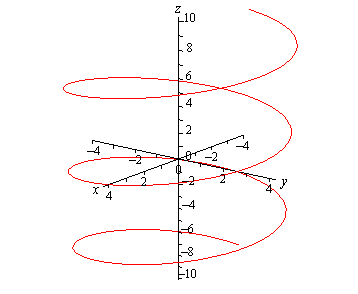
\includegraphics[scale=0.4]{curva}
		\caption{{\footnotesize Hélice de ecuación \\ $\vec{\lambda}(t)=(4cos(t),4sin(t),t)$.}}
	\end{figure}
\end{minipage}

\begin{definicion*}{Traza}
	Se llama traza del camino $f: I \subseteq R \to R^n$ al conjunto de las imágenes de $f$, es decir: traza de $f = \{f(t) \in R^n|t \in I\} \subset R^n$
\end{definicion*}

\begin{definicion*}{Curva}
	Designaremos con la palabra curva (en $R^n$) a la traza de un camino $f: I \subseteq R \to R^n$. Si el camino $f: [a,b] \to R^2,\, f(t) = (x_{t},y_{t})$ es simple, podremos decir que la curva $\{f(t) \in R^2:t \in [a,b]$\} es una \textit{curva simple}.\\
	
	Una curva es \textit{plana} si hay un plano $S$ tal que $f(t)\in S\:\forall t\in I$
\end{definicion*}

\begin{definicion*}{Curva suave}
	Curva que no posee puntos angulosos. Una curva $C$ representada por $\lambda: I \rightarrow R^{n}$ $\lambda(t) = (\lambda_1,\ldots\lambda_n)$ es suave si sus derivadas son continuas en el intervalo $I$ y no son simultáneamente nulas, excepto posiblemente en los puntos terminales del intervalo.
\end{definicion*}

\begin{definicion*}{Curva suave a trozos}
	Una curva $C$ es suave a trozos si es suave en todo intervalo de alguna partición de $I$. O sea que el intervalo puede dividirse en un número finito de subintervalos, en cada uno de los cuales $C$ es suave.
\end{definicion*}

\subsection{Diferenciabilidad. Curvas regulares}
\begin{definicion*}{Derivada de curvas regulares}
	Sea $f:I\subseteq R \to R^n$ un camino definido en el intervalo abierto I de $R$. Sea $t_0 \in I$. Se define la derivada de $f$ en $t_0$, denotada por $f^\prime(t_0)$ o $\frac{\partial f}{\partial t}(t_0)$ como el límite $f^\prime (t_0)=\lim_{h \to 0}\frac{f(t_0+h)-f(t_0)}{h}$ cuando éste existe. En tal caso se dice que el camino $f$ es diferenciable en $t_0$.\\
	
	Si la función es diferenciable en todos los puntos $t_0 \in I$, decimos que $f$ es diferenciable en $I$. Tener en cuenta que la derivada $f^\prime (t_0)$ es un vector de $R^n$, y además que éste es tangente a la curva en $t_0$, y que apunta en dirección al recorrido de la curva.
\end{definicion*}

\begin{definicion*}{Vector velocidad de curvas regulares}
	Sea $f: I \subseteq R \to R^n$ un camino diferenciable. Al vector $f^\prime(t)$ se le llama \textbf{vector velocidad} del camino en el punto $f(t) \in R^n$.
\end{definicion*}

\begin{definicion*}{Camino regular de curvas regulares}
	Sea $f: I \subseteq R \to R^3$ un camino de clase $\mathcal{C}^{1}$. $f$ es un \textbf{camino regular} si $f^\prime (t) \ne\vect{0}\:\forall t \in I.$
\end{definicion*}

\begin{definicion*}{Recta tangente de curvas regulares}
	Sea $f:I\subseteq R \to R^3$ un camino regular. \textbf{La recta tangente} a la curva en $f(t_0)$ es la recta en $R^3$ que pasa por $f(t_0)$ y tiene como vector director a uno paralelo a $f^\prime(t_0)$. Es decir:
	\begin{align}
		L:\:(x,y,z)=k(f^\prime_x(t_0),f^\prime_y(t_0),f^\prime_z(t_0))+(x(t_0),y(t_0),z(t_0))\mbox{ con \ensuremath{k\in R}}
	\end{align}
\end{definicion*}

\begin{definicion*}{Plano normal de curvas regulares}
	Para el camino $f:I\subseteq R \to R^3$ el \textbf{plano normal} a la curva correspondiente en $f(t_0)$ es el plano en $R^3$ que pasa por $f(t_0)$ y tiene por vector normal al vector $f^\prime(t_0)$. Este plano tiene como ecuación:
	\begin{align}
		\frac{\partial f}{\partial x}(t_0)(x-x(t_0))+\frac{\partial f}{\partial y}(t_0)(y-y(t_0))+\frac{\partial f}{\partial z}(t_0)(z-z(t_0))=0
	\end{align}
\end{definicion*}

\subsection{Reparametrizaciones}
\begin{definicion*}{Reparametrizaciones}
	Sea $f:[a,b] \to R^n$ un camino regular. Sea $k$ una constante positiva.\\
	
	Para recorrer la curva descrita por $f$, $k$ veces más rápido, podemos tomar la función $\varphi:[0,\frac{b-a}{k}]\to[a,b]$ dada por $\varphi(s)=ks+a$. La reparametrización será:
	\begin{align}
		\vect{f}:[0,\frac{b-a}{k}] \to R^n \text{ , } \vect{f}(s)=(f\circ\varphi)(s)=f(ks+a)
	\end{align}
	
	Si $k$ es negativa, la reparametrización recorre $f$ con una velocidad en módulo $k$ veces mayor, pero en sentido inverso al de $f$.\\
	
	Si $k=-1$, el camino $\vect{f}:[0,b-a]\to R^n$ dado por $\vect{f}(s)=f(b-s)$ recorre la curva descripta por $f$ con la misma velocidad (en módulo) de $f$, pero en sentido inverso al de $f$.
\end{definicion*}

\subsection{Longitud de un camino}
\begin{definicion*}{Rapidez de un camino}
	Llamamos \textbf{rapidez de un camino} $f:I\subseteq R \to R^n$ de clase $\mathcal{C}^{1}$ en $f(t_0)$ al número no negativo: $\left\Vert f^\prime(t_0)\right\Vert$
\end{definicion*}

\begin{definicion*}{Longitud de un camino}
	Sea $f:[a,b] \to R^n$ un camino de clase $\mathcal{C}^{1}$. La longitud de $f$ entre $t=a$ y $t=b$, denotada por $\ell(f)$, se define como:
	\begin{align}
		\ell(f)=\int_{a}^{b}\left\Vert f'(t)\right\Vert \: dt
	\end{align}
\end{definicion*}

\newpage
\section{Ecuaciones diferenciales}
\subsection{Introducción y definiciones}
\begin{definicion*}{Ecuación diferencial}
	Una ecuación se llama \emph{ecuación diferencial} si contiene derivadas o diferenciales de una o más variables dependientes de una o más variables independientes.
\end{definicion*}

\begin{definicion*}{Ecuación diferencial ordinaria}
	Son las ecuaciones diferenciales en las que figuran derivadas de diferentes órdenes de la función desconocida $y(x)$, que depende solo de una variable independiente.
\end{definicion*}

\begin{definicion*}{Orden de una ecuación diferencial}
	Se llama \emph{orden} de una ecuación diferencial al de la derivada de mayor orden que figura en dicha ecuación.\\
			
	\emph{Ejemplo}: el orden de la ecuación $y^{\prime\prime}+y^\prime=x^2$ es 2.
\end{definicion*}

\begin{definicion*}{Ecuación diferencial lineal}
	Una ecuación diferencial es \emph{lineal} cuando es lineal en $y(x)$ y en sus derivadas. Es decir que los términos que contienen la función incógnita y sus derivadas $y^\prime,y^{\prime\prime},...y^{(n)}$ aparecen como combinación lineal de $y,y^\prime,...y^{(n)}.$ Su forma general es:
	\begin{align}
		a_1(x)y+a_2(x)y^\prime+\ldots+a_n(x)y^{(n)}=f(x)
	\end{align}
\end{definicion*}

\begin{definicion*}{Problemas de valor inicial}
	Es el problema de encontrar una solución de la ecuación diferencial $y^\prime=f(x,y)$ sujeto a una condición inicial $y(x_0)=y_0$. Para que la solución a este problema sea única, debe verificarse que haya tantas condiciones iniciales como el orden de la ecuación diferencial.
\end{definicion*}

\subsection{Ecuaciones de variables separables}
\begin{definicion*}{Ecuaciones diferenciales de variables separables}
	Una ecuación diferencial separable se puede escribir de la forma $N(y)y^\prime=M(x)$.Esta ecuación se puede reescribir como:
	\begin{align}
		N(y)dy=M(x)dx
	\end{align}
	e integrando ambos miembros se obtiene una solución.
\end{definicion*}

\subsection{Ecuaciones homogéneas}
\begin{definicion*}{Ecuaciones diferenciales homogéneas}
	Son de la forma $y^\prime=f(x,y)$, donde $f(x,y)=f(tx,ty)$. Este tipo de ecuaciones se pueden resolver haciendo el cambio de variables $y=zx$, donde $z=z(x)$. Entonces reemplazamos $y^\prime$ por $z+xz^\prime$ y resolvemos.
\end{definicion*}

\subsection{Ecuaciones lineales de 1er orden}
\begin{definicion*}{Ecuaciones diferenciales lineales de orden 1}
	Sea la ecuación $y^\prime+p(x)y=q(x)$. La solución general de esta ecuación diferencial se obtiene multiplicando toda la ecuación por el factor integrante de Lagrange:
	\begin{align}
		u(x)=e^{\int p(x)dx}
	\end{align}
	Entonces la ecuación a resolver es $(u(x)y)^\prime=u(x)q(x)$.
\end{definicion*}

\subsection{Ecuaciones diferenciales exactas}
\begin{definicion*}{Ecuaciones diferenciales exactas}
	Una ecuación diferencial $P(x,y)dx+Q(x,y)dy=0$ se dice ser \emph{exacta} si exista una función $f(x,y)$ tal que la diferencial total de esta función (es decir, $df(x,y)=\frac{\partial f}{\partial x}(x,y)dx+\frac{\partial f}{\partial y}(x,y)dy$) sea:
	\begin{align}
		df(x,y)=P(x,y)dx+Q(x,y)dy
	\end{align}
	
	En el caso de que la ecuación diferencial sea exacta, la ecuación se puede escribir como $df(x,y)=0$, de modo que la familia de curvas en el plano $f(x,y)=c$ es la solución general.\\
	
	Se puede asociar la ecuación diferencial al campo vectorial $\vect{F}(x,y)=(P_{(x,y)},Q_{(x,y)})$, con lo que la propiedad de exactitud de la ecuación es equivalente a la propiedad del campo $\vect{F}$ de ser conservativo.\\

	Es decir, la ecuación es exacta si y solo si:
	\begin{align}
		\frac{\partial Q}{\partial x}=\frac{\partial P}{\partial y}
	\end{align}
\end{definicion*}

\begin{definicion*}{Factor integrante}
	Algunas ecuaciones diferenciales no exactas se pueden convertir en exactas multiplicándolas por un factor adecuado. En general, para la ecuación $P(x,y)dx+Q(x,y)dy=0$ se dice que la función no nula $\mu:U\subseteq R^2 \to R$, de clase $\mathcal{C}^{k}$, es un factor de integración si la ecuación:
	\begin{align}
		\mu P(x,y)dx+\mu Q(x,y)dy=0
	\end{align}
	En general, la función $\mu$ suele ser $\mu=\mu(x)$ o $\mu=\mu(y)$, aunque también existen $\mu=\mu(x,y)$ para ecuaciones más complicadas.
\end{definicion*}

\vspace{1cm}

\emph{Ejemplo}: Sea la ecuación $\underbrace{(3yx^2)}_{P}dx+\underbrace{(x^3+sen(y))}_{Q}dy=0$.\\

Se puede ver que $P^\prime_{y}=Q^\prime_{x}$, con lo que resulta que la ecuación es total exacta.\\

Entonces designamos $\vec{F}=(P,Q)=\nabla\phi$, con lo que resulta el sistema:

\begin{center}
	$\begin{cases}
	\phi^\prime_{x}=3yx^2 & (I)\\
	\phi^\prime_{y}=x^3+sen(y) & (II)\end{cases}\overset{integrar}{\Rightarrow}\begin{cases}
	\phi=yx^3+g(y) & (*)\\
	\phi=yx^3-cos(y)+h(x) & (\#)\end{cases}$
\end{center}

Derivando ({*}) respecto de $y$ e igualando a (II), se obtiene que:$\phi^\prime_{y}=x^3+g^\prime_{y}=x^3+sen(y)$\\

Despejando e integrando se obtiene $g(y)=-cos(y)$.\\

Entonces la solución general de la ecuación es $\phi=yx^3-cos(y)=c$.

\subsection{Trayectorias ortogonales}
\begin{minipage}{0.6\textwidth}
	\begin{definicion*}{Trayectorias ortogonales}
		Dos familias uniparamétricas de curvas $F_1(x,y,c_1)=0$ y $F_2(x,y,c_2)=0$ se dicen que son \emph{trayectorias ortogonales} si todas las curvas de una familia cortan perpendicularmente a todas las curvas de la otra familia.\\
		
		En otras palabras, en cada punto de intersección de ambas curvas la recta tangente al punto de una curva es ortogonal a la tangente de la otra curva.\\
		
		El procedimiento para hallar la familia de curvas $F_2$ ortogonales a una familia $F_1:\, y=f(x,c)$ es el siguiente:
		\begin{enumerate}
			\item Derivar la expresión de $F_1$ respecto de $x$, obteniendo $F_1^\prime:\, y^\prime=\frac{\partial f}{\partial x}$
			\item Despejar $c$ de $F_1^\prime$, y reemplazarlo en $F_1$
			\item En la nueva expresión obtenida para $F_1$ reemplazar $y^\prime$ por $-\frac{1}{y^\prime}$
			\item Resolver esta nueva ecuación diferencial.
		\end{enumerate}
		
		\underbar{Nota}: {\footnotesize Cuando la familia $F_1$ viene dada de forma implícita (ejemplo: $x^2+y^2=c$) el método es el mismo, pero se saltea	el paso 2.}
	\end{definicion*}
\end{minipage}
\begin{minipage}{0.4\textwidth}
	\begin{figure}[H]
		\centering
		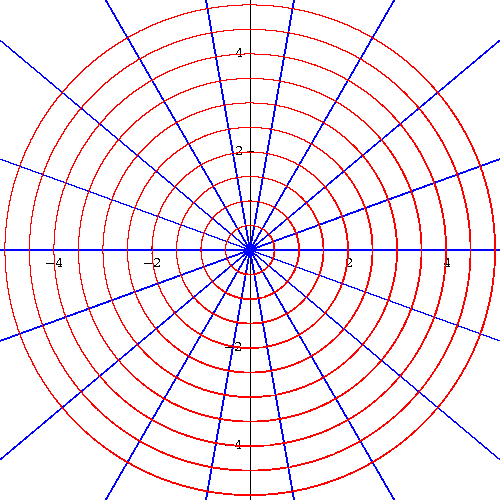
\includegraphics[scale=0.25]{curvas_ortogonales}
		\caption{{\scriptsize Círculos concéntricos (\textcolor{red}{rojo}) y \\ rectas que pasan por el origen (\textcolor{blue}{azul})}}
	\end{figure}
\end{minipage}

\newpage
\section{Integrales de línea}
\subsection{Campos vectoriales}
\begin{minipage}{0.6\textwidth}
	\begin{definicion*}{Campo vectorial}
		Una función del tipo $\vect{F}: U \subseteq R^n \to R^n$ se llama campo vectorial (en $R^n$). Este campo asocia a cada punto $x$ de $U \subseteq R^n$ el vector $\vect{F}(x)$ de $R^n$.\\
		
		Se dice que el campo vectorial $\vect{F}=(F_1,F_2,\ldots,F_n)$ es continuo (diferenciable, o de clase $\mathcal{C}^{k}$) si todas las funciones coordenadas son continuas (diferenciables, o de clase $\mathcal{C}^{k}$).
	\end{definicion*}
\end{minipage}
\begin{minipage}{0.3\textwidth}
	\begin{figure}[H]
		\centering
		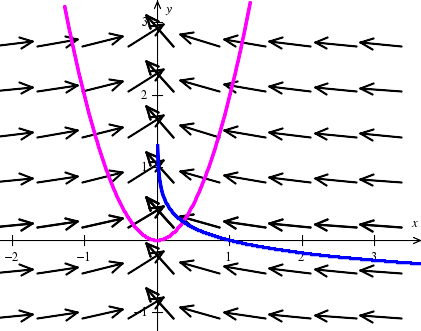
\includegraphics[scale=0.3]{lineas_de_campo}
		\caption{{\scriptsize Línea de campo (\textcolor{blue}{azul}) \\ y línea equipotencial (\textcolor{red}{rosa})}}
	\end{figure}
\end{minipage}

\begin{definicion*}{Líneas de campo}
	Para tener imágenes geométricas de campos en $R^2$, es útil considerar las \textbf{líneas de campo}. Para un campo $\vect{F}: R^2 \to R^2$, una línea de campo es una curva en $R^2$ cuya propiedad es que en cada punto de ella su tangente va en dirección al campo $\vect{F}$, es decir que $\vect{F}(\lambda(t))=\lambda^\prime(t)$.\\
	
	En general, para un campo $\vect{F}: R^n \to R^n$, las líneas de campo satisfacen que $\frac{dx_1}{F_1} = \frac{dx_2}{F_2} = \ldots = \frac{dx_n}{F_n}$.
	
	\underbar{Propiedad}: Las líneas de campo de un campo vectorial $\vect{F}$ son perpendiculares a las líneas equipotenciales (i.e. las curvas de nivel de la función potencial de $\vect{F}$).
\end{definicion*}

\begin{definicion*}{Campo de gradiente}
	Sea $f: U \subseteq R^n \to R$ diferenciable, podemos construir con ella el \textbf{campo vectorial gradiente} de $f$, $\nabla f: U \subseteq R^n \to R^n$, que asocia a cada punto $x \in U$ el vector $\nabla f(x) \in R^n$.
\end{definicion*}

\subsection{Integrales de línea sobre campo vectorial}
\begin{minipage}{0.6\textwidth}
	\begin{definicion*}{Integral de línea (circulación)}
		Sea $\vect{F}:U \subseteq R^n \to R^n,\:\vect{F}=(F_1,F_2,\ldots,F_n)$ un campo vectorial continuo, y sea $\lambda:[a,b] \to R^n,\lambda=(\lambda_1,\lambda_2,\ldots,\lambda_n)$ un camino de clase $\mathcal{C}^1$ tal que $\lambda ([a,b])\subset U$. La integral de línea del campo $\vect{F}$ a lo largo del camino $C$, o la \textbf{circulación} del campo $\vect{F}$ alrededor de (o lo largo de $\lambda$), se define como:
		\begin{align}
			\int_{\lambda} \vect{F} \cdot d\vec{l}=\int_{a}^{b} \vect{F}\left(\lambda(t)\right) \cdot \lambda^\prime(t)\: dt
		\end{align}
		
		Cuando el camino $\lambda$ es cerrado, se suele usar la notación $\oint_{\lambda} \vect{F} \cdot d\vec{l}$.

		\underbar{Una aplicación}: Si $\vect{F}$ es la fuerza que actúa sobre una partícula moviéndose a lo largo de la curva, entonces la integral sería la cantidad total de trabajo que realiza esa fuerza sobre la partícula.
	\end{definicion*}
\end{minipage}
\begin{minipage}{0.3\textwidth}
	\begin{figure}[H]
		\centering
		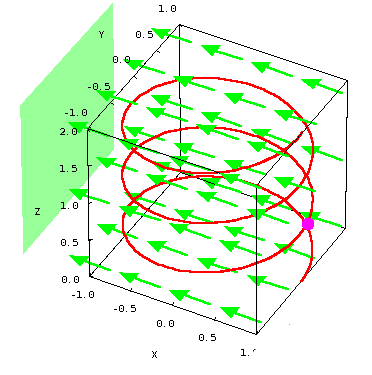
\includegraphics[scale=0.4]{integral_de_linea_de_campo_vectorial.png}
		\caption{Circulación de un campo a través de una hélice}
	\end{figure}
\end{minipage}

\begin{corolario*}{Propiedades de la Integral de línea}
	\underbar{Propiedades}:
	\begin{enumerate}
		\item $\int_{-\lambda}F\cdot d\lambda=-\int_{\lambda}F\cdot d\lambda$
		\item Una integral de línea es invariante por reparametrizaciones del camino sobre el que se integra el campo $F$.
		\item Si $F,G: U \subseteq R^n \to R^n$ son dos campos continuos y $\lambda:[a,b] \to R^n$, $\lambda \left([a,b]\right) \subset U$, un camino de clase $\mathcal{C}^1$, entonces $\int_{\lambda} \left(F+kG\right) \cdot d\lambda=\int_{\lambda}F \cdot d\lambda+k\int_{\lambda}G \cdot d\lambda$
		\item Si $\lambda=\lambda_1+\lambda_2$ entonces $\int_{\lambda}F \cdot d\lambda=\int_{\lambda_1}F \cdot d\lambda+\int_{\lambda_2}F\cdot d\lambda$
		\item Si $\mu$ es una reparametrización de $\lambda$ que conserva la orientación entonces $\int_{\mu}F \cdot d\mu=\int_{\lambda}F \cdot d\lambda$
		\item Si $\mu$ es una reparametrización de $\lambda$ que invierte la orientación entonces $\int_{\mu}F \cdot d\mu=-\int_{\lambda}F \cdot d\lambda$
	\end{enumerate}
\end{corolario*}

\subsection{Independencia del camino, campos conservativos y funciones potenciales}
\begin{teorema*}{Condiciones para de campos conservativos}
	Condición necesaria pero no suficiente para que un campo sea conservativo:\\
	
	Sea $\vect{F}:U\subseteq R^n \to R^n$, $\vect{F}=(F_1,F_2,\ldots,F_n)$ un campo de clase $\mathcal{C}^{k}(k\ge1)$ definido en el conjunto abierto $U \subseteq R^n$. Si $\vect{F}$ es conservativo entonces $\frac{\partial F_i}{\partial x_j}(x)=\frac{\partial F_j}{\partial x_i}(x)$ para $x \in U$, $1\le i<j\le n.$ Es decir que la matriz jacobiana de $\vec{F}$ debe ser simétrica.\\

	\textit{Nota}: Si la matriz es simétrica, el campo \underline{puede o no} ser conservativo. Si no lo es, podemos concluir que no es conservativo.

	\textit{Propiedad}: Si la matriz jacobiana de $\vect{F}$ es continua y simétrica en un $U$ simplemente conexo, entonces existe función potencial.
\end{teorema*}

\begin{corolario*}{Propiedades de campos conservativos}
	Sea $\vect{F}: U \subseteq R^n \to R^n$ un campo de clase $\mathcal{C}^{k}\:(k\ge0)$ definido en el conjunto abierto $U\subseteq R^n$. Las afirmaciones siguientes son equivalentes (esto es, o son todas verdaderas o todas falsas):
	\begin{enumerate}
		\item $F$ es el \emph{campo gradiente} de una función $\phi:U \subseteq R^n \to R$ de clase $\mathcal{C}^{k+1}$, es decir, $\vect{F}=\nabla\phi$
		\item La integral $\int_{\lambda} \vect{F}\: d\lambda$ a lo largo de un camino $\lambda: [a,b] \to R^n$ seccionalmente $\mathcal{C}^1$ depende solamente del punto inicial $\lambda(a)$ y final $\lambda(b)$ del camino $\lambda$: $\int_{\lambda} \vec{F} \cdot d\lambda=\phi(b)-\phi(a)$
		\item La integral $\int_{\lambda}\vect{F}\: d\lambda$ a lo largo de un camino $\lambda:[a,b] \to R^n$ cerrado seccionalmente $\mathcal{C}^1$ es cero.
		\item El campo $\vect{F}$ es \textit{conservativo}.
		\item La función $\phi: U \subseteq R^n \to R$ de clase $\mathcal{C}^{k+1}$ es la \textit{función potencial}.
	\end{enumerate}
\end{corolario*}

\subsection{Integrales de línea de campo escalar}
\begin{definicion*}{Integral de línea}
	Sea $f: U \subseteq R^n \to R$ una función real continua definida en el abierto $U \subseteq R^n$, y sea $\lambda:[a,b] \to R^n$ un camino de clase $\mathcal{C}^1$ tal que $\lambda\left([a,b]\right)\subset U$.\\

	La integral de línea respecto a la longitud de arco de la función $f$ a lo largo del camino $\lambda$ es:
	\begin{align}
		\int_{\lambda}\, f\: dl=\int_{a}^{b}f\left(\lambda(t)\right) \cdot \left\Vert \lambda^\prime(t) \right\Vert dt
	\end{align}
	Donde $dl=\left\Vert \lambda^\prime(t) \right\Vert dt$ es la diferencial de la longitud de arco del camino $\lambda$.\\

	\underbar{Una aplicación}: Conociendo la densidad lineal de un alambre en el espacio, digamos que dada por la función $\rho=\rho(x,y,z)$ (en gr/cm), y el camino $C:[a,b] \to R^3$ en cuya imagen \emph{se encuentra el alambre}, entonces su masa total se calcula como $M=\int_{C} \rho\: dl$.
\end{definicion*}

\begin{corolario*}{Propiedades de Integraesl de línea}
	\begin{enumerate}
		\item Si $f,g: U \subseteq R^n \to R$ son dos funciones continuas definidas en el abierto $U \subseteq R^n$ y $C:[a,b] \to R^n$ es un camino seccionalmente $\mathcal{C}^1$, entonces:
			\begin{align}
				\int_{C} (f+kg) \cdot ds=\int_{C}f \cdot ds+k\int_{C}g \cdot ds
			\end{align}
		\item Sea $f: U \subseteq R^n \to R$ una función continua definida en el abierto $U \subseteq R^n$. Sea $\lambda:[a,b] \to R^n$ un camino de clase $\mathcal{C}^1$ tal que $\lambda \left([a,b]\right) \subset U$, y sea $\mu:[c,d] \to R^n$ una reparametrización de $\lambda$. Entonces $\int_{\lambda}f\: ds=\int_{\mu}f\: ds$.
	\end{enumerate}
\end{corolario*}

\subsection{La perspectiva de la física}
\begin{corolario*}{Trabajo}
	Sea $\vect{F}: U \subseteq R^2$ (o $R^3$) $ \to R^2$ (o $R^3$) un campo de clase $\mathcal{C}^{k}$, $k\ge0$, y sea $\lambda:[a,b] \to R^2$ (o $R^3$) un camino seccionalmente $\mathcal{C}^1$ cuya imagen está contenida en $U$. El trabajo que hay que realizar para llevar un cuerpo de masa $m$ del punto $p=\lambda(a)$ al punto $q=\lambda(b)$ por el camino $\lambda$ a través del campo $\vect{F}$ es:\\
	\begin{align}
		W_{pq}=\int_{\lambda} \vect{F} \cdot d\lambda=\int_{a}^{b} \vect{F} \left(\lambda(t)\right) \cdot \lambda^\prime(t)dt=m\int_{a}^{b}\lambda^{\prime\prime}(t) \cdot \lambda^\prime (t)dt=\frac{1}{2}m\left|\lambda^\prime(b)\right|^2-\frac{1}{2}m\left|\lambda^\prime(a)\right|^2
	\end{align}
\end{corolario*}

\begin{corolario*}{Teorema del valor medio}
	Sea una función continua $f: U \subseteq R^n \rightarrow R$ definida en el abierto $U$ de $R^n$, y un camino de clase $\mathcal{C}^1 \text{ } \lambda:[a,b] \rightarrow R^n \text{ , } \lambda([a,b])\subset U$, definimos el valor medio de la función $f$ sobre el camino $\lambda$, como:
	\begin{align}
		\bar{f}_{\lambda}=\frac{1}{L_{\lambda}} \cdot \int_{\lambda}\, f\, dl=\frac{1}{\int_{a}^{b}\left\Vert \lambda^\prime(t)\right\Vert dt} \cdot \int_{a}^{b}f(\lambda(t)) \cdot \left\Vert \lambda^\prime(t)\right\Vert dt
	\end{align}
	
	El valor $\bar{f}$ es un tipo de promedio de los valores que toma la función a lo largo del camino $\lambda$.
\end{corolario*}

\newpage
\section{Integrales múltiples}
\subsection{Integrales dobles}
\begin{definicion*}{Integral doble}
	Sea $f: Q \subset R^2 \to R$ una función escalonada definida en el rectángulo Q de $R^2$. Digamos que $Q$ está dividido en $nm$ subrectángulos $Q_{ij}$.\\
	
	Se define la integral doble de la función $f(x,y)$ sobre el rectángulo $Q$, como: 
	\begin{align}
		\iint_{Q} f(x,y)\: dxdy=\sum_{i=1}^{n} \sum_{j=1}^{m} c_{ij} (x_i-x_{i-1}) (y_j-y_{j-1})
	\end{align}
	Notar que si $f(x,y)=k$ para $(x,y) \in Q=[a,b] \times [c,d]$ se tiene $\iint_{Q} f(x,y)dxdy=k\cdot(\acute{a}rea\: de\: Q)$.\\
	
	Si $k>0$, el valor de la integral representa el volumen de un paralepípedo rectangular con base Q y altura $k$.
\end{definicion*}

\begin{teorema*}{Teorema para Integral doble}
	Si la función $f: Q \subset R^2 \to R$ definida en el rectángulo $Q=[a,b] \times [c,d]$ es continua, entonces es integrable, y la integral doble de ella sobre $Q$ se puede calcular como:
	\begin{align}
		\iint_{Q} f(x,y)\: dxdy=\int_{c}^{d} \left(\int_{a}^{b} f(x,y)dx\right)dy=\int_{a}^{b}\left(\int_{c}^{d} f(x,y)\, dy\right)\, dx
	\end{align}
	De forma geométrica, la integral doble de la función $f(x,y)$ sobre $Q$ es el volumen del paralepípedo cuya tapa es la gráfica de la función $f(x,y)$ sobre $Q$. Consideremos el cuerpo $\Omega$ que queda limitado entre la gráfica de $f(x,y)$, el plano $xy$ y el área limitada por $Q$. Entonces se tiene que:
	\begin{align}
		\iint_{Q}f(x,y)\, dxdy=\text{ volumen de }\Omega
	\end{align}
\end{teorema*}

\subsection{Integrales dobles de funciones sobre regiones más generales}
\begin{definicion*}{Regiones tipo I}
	\textbf{Regiones del tipo (I)} son regiones limitadas:
	
	\begin{minipage}{0.3\textwidth}
		\begin{figure}[H]
			\centering
			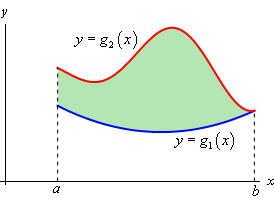
\includegraphics[scale=0.4]{tipo1}
		\end{figure}
	\end{minipage}
	\begin{minipage}{0.7\textwidth}
		\begin{enumerate}
			\item por la recta vertical $x=a$ por la izquierda,
			\item por la recta vertical $x=b$ por la derecha,
			\item por la gráfica de la función de $x$, $y=g_1(x)$ por debajo,
			\item por la gráfica de la función de $x$, $y=g_2(x)$ por encima.
		\end{enumerate}
	\end{minipage}
\end{definicion*}

\begin{definicion*}{Regiones tipo II}
	\textbf{Regiones del tipo (II)} son regiones limitadas:
	
	\begin{minipage}{0.25\textwidth}
		\begin{figure}[H]
			\centering
			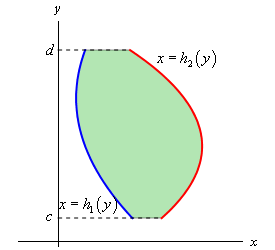
\includegraphics[scale=0.35]{tipo2}
		\end{figure}
	\end{minipage}
	\begin{minipage}{0.75\textwidth}
		\begin{enumerate}
			\item por la recta horizontal $y=c$ por debajo,
			\item por la recta horizontal $y=d$ por encima,
			\item por la gráfica de la función de $y$, $x=h_1(y)$ por la izquierda,
			\item por la gráfica de la función de $y$, $x=h_2(y)$ por la derecha.
		\end{enumerate}
	\end{minipage}
\end{definicion*}

\begin{definicion*}{Regiones tipo III}
	\textbf{Regiones del tipo (III)}: Son aquellas regiones que debemos dividir para verlas como la unión de varias regiones de tipo (I) o tipo (II).\\

	Sea $f: R \subset R^2 \to R$. Si la región R es de tipo (I), es decir, si $R = \{(x,y):\, a \le x \le b,\,\phi_1(x) \le y\le \phi_2(x)\}$ entonces la integral doble de $f(x,y)$ sobre $R$ se puede calcular como: 
	\begin{align}
		\iint_{R} (x,y)\, dxdy=\int_{a}^{b} \left(\int_{\phi_1(x)}^{\phi_2(x)}f(x,y)\, dy\right)dx.
	\end{align}

	Si la región $R$ es de tipo (II), es decir, si $R=\{(x,y):\,\psi_1(y)\le x\le\psi_2(y),\, c\le y\le d\}$, entonces la integral doble de $f(x,y)$ sobre $R$ se puede calcular como: 
	\begin{align}
		\iint_{R} f(x,y)dxdy=\int_{c}^{d}\left(\int_{\psi_1(y)}^{\psi_2(y)} f(x,y)dx\right)dy.
	\end{align}
\end{definicion*}

\begin{corolario*}{Propiedades de integrales dobles}
	Si la región $R$ está subdividida en dos subregiones $R_1$ y $R_2$ (es decir, $R=R_1 \cup R_2$), entonces:
	\begin{align}
		\iint_{R} f(x,y)\, dxdy=\iint_{R_1} f(x,y)\, dxdy+\iint_{R_2} f(x,y)\, dxdy
	\end{align}
\end{corolario*}

\subsection{Cambio de variable en integrales dobles}
\begin{teorema*}{Teorema de cambio de variable}
	Sea $f: R \subset R^2 \to R$ una función continua de las variables $x,y$ definida en la región $R \subset R^2$.\\
	Sea $F:R^\prime \subset R^2 \to R$, $F(u,v)=(\phi_{(u,v)},\psi_{(u,v)})$ una función que manda de manera inyectiva los puntos $(u,v)\in R^\prime$ en los puntos $(x,y)\in R$ del plano $xy$. Si $F \in \mathcal{C}^1$ y la derivada $F^\prime(u,v)$ es una matriz inversible para todo $(u,v) \in R^\prime$, entonces la fórmula de cambio de variables en integrales dobles es:
	\begin{align}
		\iint_{R}f(x,y)\, dxdy=\iint_{R^\prime}f\left(\phi(u,v),\psi(u,v)\right) \cdot \left|\frac{\partial(\phi,\psi)}{\partial(u,v)}\right|dudv
	\end{align}
	En general, cuando en la región de integración se presentan anillos circulares, y/o cuando en la función a integrar aparezca de alguna forma las expresiones $\left(x^2+y^2\right),\frac{y}{x}$ puede resultar conveniente intentar el cálculo de la integral haciendo previamente el cambio a coordenadas polares:
	$\begin{cases}
		x=rcos(\theta)\\
		y=rsin(\theta)
	\end{cases}$.
	En este caso, el jacobiano de la transformación que aparece en la fórmula de cambio de variables es $\frac{\partial (x,y)}{\partial (r,\theta)}=r$.
	Entonces la fórmula es:
	\begin{align}
		\iint_{R}f(x,y)\: dxdy=\iint_{R'}f\left(rcos(\theta),rsin(\theta)\right)\cdot r\: drd\theta
	\end{align}
\end{teorema*}

\subsection{Aplicaciones de las integrales dobles}
\begin{minipage}{0.6\textwidth}
	\begin{corolario*}{Cálculo de volumen}
		El volumen $V$ encerrado entre una superficie $z=f(x,y)$ ($>0$) y una región $R$ en el plano $xy$ es:
		\begin{align}
			V=\iint_{R}f\left(x,y\right)\: dxdy
		\end{align}
	\end{corolario*}
\end{minipage}
\begin{minipage}{0.3\textwidth}
	\begin{figure}[H]
		\centering
		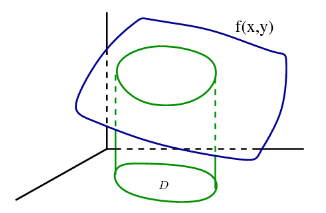
\includegraphics[scale=0.3]{integral_doble_es_volumen.png}
		\caption{Volumen bajo la\\ gráfica de $f(x,y)$}
	\end{figure}
\end{minipage}

\begin{corolario*}{Cálculo de área}
	El área de una región plana $R$ en el plano $xy$ viene dada por una integral doble:
	\begin{align}
		area (R)=\iint_{R}\: dxdy
	\end{align}
\end{corolario*}

\begin{corolario*}{Cálculo de masa total}
	Sea $\rho(x,y)$ la función de densidad (igual a masa por unidad de área) de una distribución de masa en el plano $xy$. Entonces la masa total de un trozo plano $R$ es:
	\begin{align}
		M=\iint_{R}\rho\left(x,y\right)\: dxdy
	\end{align}
\end{corolario*}

\begin{corolario*}{Centro de masa y momentos de figuras planas}
	\begin{center}
		Momentos estáticos =$\left\{ \begin{array}{c}
		M_{x}=\iint_{R}y\cdot\rho\left(x,y\right)\: dxdy\\
		M_{y}=\iint_{R}x\cdot\rho\left(x,y\right)\: dxdy\end{array}\right.$
		\begin{align}
			CM=\left(\overline{x},\overline{y}\right)=\left(\frac{M_{x}}{M},\frac{M_{y}}{M}\right)
		\end{align}
		\par
	\end{center}
\end{corolario*}

\subsection{Integrales triples}
\begin{teorema*}{Teorema para integrales triples}
	Sea $f: Q \subset R^3 \to R$ una función continua definida en el rectángulo $Q=[a,b] \times [c,d] \times [e,g]$ de $R^3$. Entonces $f$ es integrable en $Q$ y:
	\begin{align}
		\iiint_{Q} f(x,y,z)\: dxdydz=\int_{a}^{b}\int_{c}^{d}\left(\int_{e}^{g}f\left(x,y,z\right)\, dz\right)dydx
	\end{align}
	Las regiones que se pueden presentar serán, en general, subconjuntos de $R^3$ limitados por gráficas de funciones de dos variables.\\
	De modo más preciso, si $R$ es una región del plano $xy$, definamos	$\Omega$ como:
	\begin{align}
		\Omega=\{\bar{x}\in R^3:(x,y)\in R\:\wedge\:\phi_{1}(x,y)\leq z\leq\phi_{2}(x,y)\}
	\end{align}
	Donde $\phi_1,\phi_2$ son funciones continuas definidas en la región $R$ de $R^2$. Más aún, esta integral se calcula como:
	\begin{align}
		\iiint_{\Omega}f(x,y,z)\, dxdydz=\iint_{R}\left[\int_{\phi_1}^{\phi_2}f(x,y,z)\, dz\right]dxdy
	\end{align}
	La integral triple de $f(x,y,z)$ sobre $\Omega$ es la integral doble de una función $\xi(x,y)$ sobre la región $R$, la cual se puede ver como \emph{la proyección de la región $\Omega$ sobre el plano $xy$}. Esta proyección se obtiene expresando el cuerpo en función de las variables $x,y$. También se pueden considerar regiones $R$ en el plano $xz$ e $yz$.
\end{teorema*}

\subsection{Cambio de variable en integrales triples}
\begin{teorema*}[0.9\textwidth]{Teorema de cambio de variable}
	Consideremos una función de transformación de coordenadas $F:\Omega^\prime \subset R^3 \to R^3$ del tipo $F(u,v,w)=(x,y,z)=\left(x_{(u,v,w)},y_{(u,v,w)},z_{(u,v,w)}\right).$	La fórmula de cambio de cambio de variables en integrales triples es:
	\begin{align}
		\iiint_{\Omega}f(x,y,z)\: dxdydz=\iiint_{\Omega'}f\left(F(u,v,w)\right)\left|\frac{\partial(x,y,z)}{\partial(u,v,w)}\right|dudvdw
	\end{align}
	\begin{itemize}
		\item \textbf{Coordenadas cilíndricas}: Son útiles cuando aparecen cilindros o planos:
			\begin{align}
				\iiint_{\Omega} f \left(x,y,z\right)\: dxdydz = \iiint_{\Omega'} f \left(rcos(\theta), rsin(\theta), z\right) \cdot r\: drd\theta dz
			\end{align}
		\item \textbf{Coordenadas cilíndricas generalizadas}:
			\begin{align}
				\iiint_{\Omega} f \left(x,y,z\right)\: dxdydz = \iiint_{\Omega'} f \left(a \cdot rcos(\theta), b \cdot rsin(\theta), c\widetilde{z}\right) \cdot abcr\: drd\theta dz
			\end{align}
		\item \textbf{Coordenadas esféricas}:
			\begin{small}
				\begin{align}
				\iiint_{\Omega} f \left(x,y,z\right)\: dxdydz = \iiint_{\Omega'} f \left(rcos(\theta) sin(\phi), rsin(\theta) sin(\phi), rcos(\phi)\right) \cdot r^{2}sin(\phi)\: drd\theta d\phi
				\end{align}
			\end{small}
		\item \textbf{Coordenadas esféricas generalizadas}:
			\begin{footnotesize}
				\begin{align}
					\iiint_{\Omega} f(x,y,z)\: dxdydz = \iiint_{\Omega'} f (a \cdot rcos(\theta) sin(\phi),b \cdot sin(\theta) sin(\phi), c \cdot rcos(\phi)) \cdot abcr^{2}sin(\phi)\: drd\theta d\phi
				\end{align}
			\end{footnotesize}
	\end{itemize}
\end{teorema*}

\subsection{Aplicaciones de las integrales triples}
\begin{corolario*}{Cálculo de volúmenes en el espacio}
	El volumen $V$ de un cuerpo de superficie $f(x,y,z)$ es:
	\begin{align}
		V=\iiint_{\Omega}\, dxdydz
	\end{align}
\end{corolario*}

\begin{corolario*}{Cálculo de masa de cuerpos en el espacio}
	Sea $d(x,y,z)$ la función densidad, y $\Omega \in R^3$. Entonces:
	\begin{align}
		M=\iiint_{\Omega}d(x,y,z)\: dxdydz=\mbox{masa de \ensuremath{\Omega}}
	\end{align}
\end{corolario*}

\begin{corolario*}{Cálculo de centros de masa y momentos de cuerpos en el espacio}
	\begin{align}
		\text{Momentos estáticos:}
		=\begin{cases}
		M_{xy}=\iiint_{\Omega}z\cdot d(x,y,z)\, dxdydz\\
		M_{xz}=\iiint_{\Omega}y\cdot d(x,y,z)\, dxdydz\\
		M_{yz}=\iiint_{\Omega}x\cdot d(x,y,z)\, dxdydz\end{cases}
	\end{align}
	\begin{align}
		\text{Centro de masa}=(\bar{x},\bar{y},\bar{z})=\left(\frac{M_{yz}}{M},\frac{M_{xz}}{M},\frac{M_{xy}}{M}\right)
	\end{align}
\end{corolario*}

\newpage
\section{Integrales de superficie}
\subsection{Superficies simples}
\begin{minipage}{0.6\textwidth}
	\begin{tikzpicture}
		\node[definicion](box){
			\begin{minipage}{0.8\textwidth}
				Una curva es un objeto unidimensional en $R^2$ o $R^3$, es decir, una curva es la imagen de una cierta función definida \textit{en un subconjunto I} de la recta (espacio de dimensión 1). De la misma manera, una superficie será la imagen en $R^3$ de una cierta función que está definida en \textit{un subconjunto $D$ de } $R^2$ (que es bidimensional).
			\end{minipage}};
		\node[fancytitle, right=10pt] at (box.north west) {Curvas};
		\node[fancytitle, rounded corners] at (box.south) {$\aleph$};
	\end{tikzpicture}
\end{minipage}
\begin{minipage}{0.3\textwidth}
	\begin{figure}[H]
		\begin{center}
			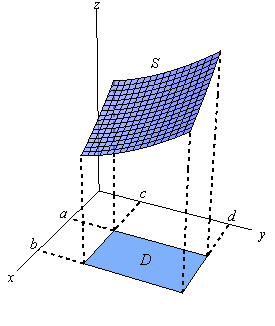
\includegraphics[scale=0.3]{integrales_de_sup.png}{\small \caption{Superficie simple}}
		\end{center}
	\end{figure}
\end{minipage}

\begin{tikzpicture}
	\node[definicion](box){
		\begin{minipage}{0.8\textwidth}
			Sea $S \subseteq R^2$ una región del tipo I y del tipo II en $R^2$, y sea $f: S \subset R^2 \to R^3$, $f(u,v)=(f_{1(u,v)},f_{2(u,v)},f_{3(u,v)})$ una función inyectiva (para que no haya puntos tales que $f(p_1)=f(p_2) \in K$) de clase $C^1$, de modo que los vectores $\frac{\partial f}{\partial u}$ y $\frac{\partial f}{\partial v}$ son linealmente independientes en todo $(u,v)\in S$.\\
			
			A la imagen de la función $f$, $K=f(S)$, se le llama superficie simple. La región $S$, dominio de $f$, es una región cerrada y acotada del plano $R^2$.\\

			\emph{Notación:} $\partial K$ es la frontera de K ($\partial K=f(\partial S)$ con $\partial S$ la frontera de S, su dominio), e $\text{Int}(K)$ es el interior de de la superficie simple $K$, siendo $\text{Int}(K)=f(\text{Int},S)$.
		\end{minipage}};
	\node[fancytitle, right=10pt] at (box.north west) {Superficie simple};
	\node[fancytitle, rounded corners] at (box.south) {$\aleph$};
\end{tikzpicture}

\begin{tikzpicture}
	\node[definicion](box){
		\begin{minipage}{0.8\textwidth}
			Dada la superficie de ecuación $\bar{x}=\vect{F}(u,v)$ con $(u,v)\in D$, se dice que la misma es \emph{regular} si:
			\begin{align}
				\vect{F}  \text{ es diferenciable y }\\
				\vect{F}^\prime_u,\vect{F}^\prime_v \neq0
			\end{align}
		\end{minipage}};
	\node[fancytitle, right=10pt] at (box.north west) {Superficie regular};
	\node[fancytitle, rounded corners] at (box.south) {$\aleph$};
\end{tikzpicture}

\begin{tikzpicture}
	\node[definicion](box){
		\begin{minipage}{0.8\textwidth}
			Dada la superficie de ecuación $\vect{x}=\vect{F}(u,v)$ con $(u,v) \in D$, se dice que la misma es \emph{suave} si:
			\begin{align}
				\vect{F}(u,v) \text{ es regular y }\\
				\vect{F}(u,v) \in C^2
			\end{align}
			Intuitivamente, una superficie suave no tiene \emph{esquinas}.
		\end{minipage}};
	\node[fancytitle, right=10pt] at (box.north west) {Superficie suave};
	\node[fancytitle, rounded corners] at (box.south) {$\aleph$};
\end{tikzpicture}

\subsection{Orientación de superficies}
\begin{tikzpicture}
	\node[definicion](box){
		\begin{minipage}{0.8\textwidth}
			De manera general, una superficie $K$ en $R^3$ se dirá \emph{orientable} si es posible decidir sin ambigüedad cuál es cada uno de los lados de la superficie, el \emph{interior} y el \emph{exterior}.\\
			
			Decir que una superficie $K$ es orientable, significa que podemos tener un campo de vectores normales a $K$, $N:K \to R^3$, de manera que los vectores normales apunten en la dirección de uno de los lados de la superficie. Se requiere que este campo $N$ sea continuo en $K$. Este campo es $N(x,y,z)=\frac{\frac{\partial f}{\partial u}\times\frac{\partial f}{\partial v}}{\left\Vert \frac{\partial f}{\partial u}\times\frac{\partial f}{\partial v}\right\Vert }$.\\
			
			Para obtener un vector normal a una superficie, se utiliza la \emph{regla	del pulgar:} si imaginamos que caminamos alrededor de $\partial S$, la superficie debe quedar a nuestra izquierda, y nosotros seríamos el vector normal $\breve{n}$.\\
		\end{minipage}};
	\node[fancytitle, right=10pt] at (box.north west) {Orientación de superficies};
	\node[fancytitle, rounded corners] at (box.south) {$\aleph$};
\end{tikzpicture}

\emph{Ejemplo(superficie implícita):} Tenemos una superficie $S$ dada por $z=4-x^{2}$ y queremos obtener un vector normal en un punto $(x_{0},y_{0},z_{0})$.\\

Si tomamos $\vect{F}(x,y,z)=z-4+x^{2}$, sabemos que la superficie $S$ es la curva de nivel $0$ de $F$, y por lo tanto es perpendicular al gradiente de $\vect{F}$, que a su vez es paralelo al vector normal.\\

Entonces $\nabla F=(2x,0,1)$, y tenemos que el vector normal al punto es $(2x_0,0,1)$.

\subsection{Área de una superficie }
\begin{tikzpicture}
	\node[definicion](box){
		\begin{minipage}{0.8\textwidth}
			Sea $S=f(D)$ una superficie simple en $R^3$ parametrizada por la función $f:D \subset R^2 \to R^3$. El área de la superficie $\Sigma$ se define como:
			\begin{align}
				\mbox{Area de S}=\iint_{D}\left\Vert \frac{\partial f}{\partial u}\times\frac{\partial f}{\partial v}\right\Vert \, dudv
			\end{align}
	
			\underbar{Nota}: El área de la superficie $S$ es independiente de la parametrización que se tenga de ella.
		\end{minipage}};
	\node[fancytitle, right=10pt] at (box.north west) {Área de superficies};
	\node[fancytitle, rounded corners] at (box.south) {$\aleph$};
\end{tikzpicture}

\subsection{Integrales de superficie de campos escalares}
\begin{tikzpicture}
	\node[definicion](box){
		\begin{minipage}{0.8\textwidth}
			Sea $S$ una superficie simple parametrizada por la función $\phi: D \subset R^2 \to R^3$, $\phi(u,v)=(\phi_1,\phi_2,\phi_3)$. Sea $f: S \to R$ una función escalar continua definida sobre la superficie $S$. La integral de superficie de la función $f$ sobre $S$ se define como:
			\begin{align}
				\iint_{S}f\, ds=\iint_{S}f(\phi(u,v))\cdot\left\Vert \frac{\partial\phi}{\partial u}\times\frac{\partial\phi}{\partial v}\right\Vert \, dudv
			\end{align}
	
			\underbar{Nota}: Si $f(x,y,z)=1$, la integral $\iint_{S}\, f\, ds$ no es más que la definición de área de la superficie $S$.\\

			\underbar{Una aplicación}: Si la función $f$ representa la densidad de una sábana, la integral sería la masa total de la sábana.
		\end{minipage}
		};
	\node[fancytitle, right=10pt] at (box.north west) {Integral de superficie en campo escalar};
	\node[fancytitle, rounded corners] at (box.south) {$\aleph$};
\end{tikzpicture}

\subsection{Integrales de superficie de campos vectoriales}
\begin{minipage}{0.3\textwidth}
	\begin{figure}[H]
		\begin{center}
			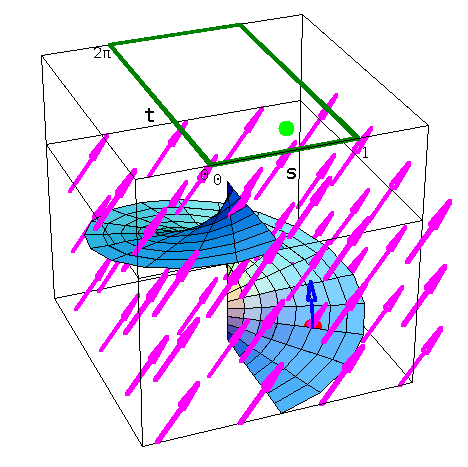
\includegraphics[scale=0.24]{integral_de_superficie.png}\caption{Integral de superficie.}
		\end{center}
	\end{figure}
\end{minipage}
\begin{minipage}{0.6\textwidth}
	\begin{tikzpicture}
		\node[definicion](box){
			\begin{minipage}{0.8\textwidth}
				Sea $S$ una superficie simple parametrizada por la función $\phi: D \subset R^2 \to R^3$, $\phi(u,v)=(\phi_1,\phi_2,\phi_3)$ la cual proporciona una orientación que coincide con la del campo continuo de vectores normales $N: S \to R^3$. Sea $\vect{F}: U \subseteq R^3 \to R^3$ un campo continuo definido en el abierto $U$ de $R^3$ que contiene a $S$. Se define la integral de superficie de $\vect{F}$ sobre $S$, llamada flujo de $\vect{F}$ a través de $S$, como
				\begin{align}
					\iint_{S}\vect{F}\cdot d\vect{s}=\iint_{D}\vect{F}(\phi(u,v)) \cdot \left(\frac{\partial\phi}{\partial u}\times\frac{\partial\phi}{\partial v}\right)\, dudv
				\end{align}
				
				\underbar{Nota}: La integral es invariante por reparametrizaciones que no cambian la orientación de la superficie $S$. Si tomamos una reparametrización de $S$ que cambie su orientación, esto sí se reflejará en un cambio de signo de la integral.\\
			
				\underbar{Una aplicación}: Si el campo vectorial $\vect{F}$ representa el flujo de un líquido, entonces la integral de superficie de $\vect{F}$ representa la cantidad de fluido que fluye a través de la superficie $S$ por unidad de tiempo.
			\end{minipage}};
		\node[fancytitle, right=10pt] at (box.north west) {Flujo};
		\node[fancytitle, rounded corners] at (box.south) {$\aleph$};
	\end{tikzpicture}
\end{minipage}

\newpage
\section{Teoremas integrales}
\subsection{Gradiente, Divergencia, Rotor: las fórmulas clásicas}
\begin{tikzpicture}
	\node[definicion](box){
		\begin{minipage}{0.8\textwidth}
			Sea $f$ un campo escalar y $\vect{F}=(P,Q,R)$ un campo vectorial:
			\begin{align}
				\nabla=\left(\frac{\partial}{\partial x_1},\frac{\partial}{\partial x_2},\cdots,\frac{\partial}{\partial x_n}\right) \in R^n \\
				\nabla \cdot f=\text{grad}(f)=\left(\frac{\partial f}{\partial x_1},\frac{\partial f}{\partial x_2},\cdots,\frac{\partial f}{\partial x_n}\right) \\
				\nabla \cdot \vect{F}=\text{div}\left(\vect{F}\right)=P_x^\prime+Q_y^\prime+R_z^\prime=\text{tr}\left(J(\vect{F})\right) \\
				\nabla \times \vect{F}=\text{rot} \left(\vect{F}\right)=\left(\frac{\partial R}{\partial y}-\frac{\partial Q}{\partial z},\frac{\partial R}{\partial x}-\frac{\partial P}{\partial z},\frac{\partial Q}{\partial x}-\frac{\partial P}{\partial y}\right) \\
				\nabla \cdot \nabla f=\text{div}(\text{grad}(f))=\frac{\partial^2 f}{\partial x_1^2}+\frac{\partial^2 f}{\partial x_2^2}+\ldots+\frac{\partial^2 f}{\partial x_n^2}=\nabla^2 f=\text{Laplaciano de \ensuremath{f}}
			\end{align}
		\end{minipage}};
	\node[fancytitle, right=10pt] at (box.north west) {Fórmulas: Gradiente,Divergencia, Rotor};
	\node[fancytitle, rounded corners] at (box.south) {$\aleph$};
\end{tikzpicture}

\begin{tikzpicture}
	\node[corolario](box){
		\begin{minipage}{0.8\textwidth}
			\begin{align}
				\text{div}(\text{rot}(\vect{F}))=0 \Rightarrow \text{ Campo selenoidal} \\
				\text{rot}(\text{grad}(f))=0 \Rightarrow \text{ Campo irrotacional} \\
				\text{div}(\text{grad}(f)\times \text{grad}(g))=0 \Rightarrow \text{ Campo selenoidal} \\
				\nabla^2 f=\text{div}(\text{grad}(f))=0 \Rightarrow \text{ Función armónica}
			\end{align}
		\end{minipage}};
	\node[fancytitle, right=10pt] at (box.north west) {Propiedades};
	\node[fancytitle, rounded corners] at (box.south) {$\aleph$};
\end{tikzpicture}

\begin{tikzpicture}
	\node[definicion](box){
		\begin{minipage}{0.8\textwidth}
			Se dice que la función $f: U \subseteq R^n \to R$ de clase $\mathcal{C}^2$ definida en $U$, es \textbf{armónica} si satisface la ecuación de Laplace:
			\begin{align}
				\nabla^{2}f=0
			\end{align}
			Es decir, si:
			\begin{align}
				\sum_{i=1}^{n}\frac{\partial^2 f}{\partial x_i^{2}}=0
			\end{align}
		\end{minipage}};
	\node[fancytitle, right=10pt] at (box.north west) {Función armónica};
	\node[fancytitle, rounded corners] at (box.south) {$\aleph$};
\end{tikzpicture}

\begin{tikzpicture}
	\node[definicion](box){
		\begin{minipage}{0.8\textwidth}
			Un campo vectorial $\vect{F}$ se dice \textbf{solenoidal} si:
			\begin{align}
				div(\vect{F})\equiv0 \text{ ,para todo punto del dominio.}
			\end{align} 
			La integral de superficie o flujo de un campo solenoidal sobre cualquier superficie cerrada es siempre cero. Los campos solenoidales no tienen ni puntos fuentes ($div(\vec{F})>0$) ni puntos sumideros ($div(\vec{F})<0$).
		\end{minipage}};
	\node[fancytitle, right=10pt] at (box.north west) {Campo senoidal};
	\node[fancytitle, rounded corners] at (box.south) {$\aleph$};
\end{tikzpicture}

\begin{tikzpicture}
	\node[definicion](box){
		\begin{minipage}{0.8\textwidth}
			Un campo vectorial $\vect{F}$ se dice \textbf{irrotacional} si:
			\begin{align}
				\text{rot}(\vect{F})\equiv 0
			\end{align}
			Para todo punto del dominio. Un campo es irrotacional si y sólo si su matriz jacobiana es simétrica en un dominio convexo. Esto quiere decir que el campo es conservativo, y por lo tanto admite función potencial, por lo que la integral de línea sobre cualquier curva cerrada es cero siempre.
		\end{minipage}
		};
	\node[fancytitle, right=10pt] at (box.north west) {Campo irrotacional};
	\node[fancytitle, rounded corners] at (box.south) {$\aleph$};
\end{tikzpicture}

\subsection{Rotor de un campo vectorial}
\begin{minipage}{0.25\textwidth}
	\begin{figure}[H]
		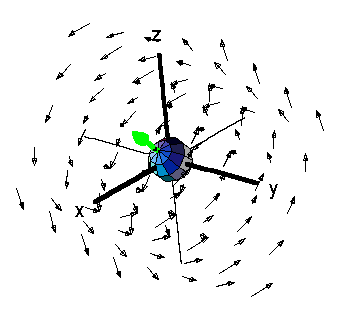
\includegraphics[scale=0.3]{rotor}\caption{{\footnotesize El rotor de un \\campo (en \textcolor{green}{verde})}}
	\end{figure}
\end{minipage}
\begin{minipage}{0.7\textwidth}
	\begin{tikzpicture}
		\node[definicion](box){
			\begin{minipage}{0.9\textwidth}
				Sea $\vect{F}: U \subseteq R^3 \to R^3$, $\vect{F}=(F_1,F_2,F_3)$ diferenciable, definido en $U$. Se define el \emph{rotor} (o \textbf{rotacional}) de $\vect{F}$ en el punto $p \in U$, como:
				\begin{small}
					\begin{align}
						rot(\vec{F})=\left|\begin{array}{ccc} \hat{i} & \hat{j} & \hat{k} \\\frac{\partial}{\partial x} & \frac{\partial}{\partial y} & \frac{\partial}{\partial z}\\
						F_{1} & F_{2} & F_{3}\end{array}\right|=\left(\frac{\partial F_{3}}{\partial y}-\frac{\partial F_{2}}{\partial z},\frac{\partial F_{1}}{\partial z}-\frac{\partial F_{3}}{\partial x},\frac{\partial F_{2}}{\partial x}-\frac{\partial F_{1}}{\partial y}\right)
					\end{align}
				\end{small}
				
				Geométricamente, el rotacional de $\vect{F}$ es un vector que apunta al eje de rotación, y su longitud corresponde a la velocidad de rotación.\\
				
				Un resultado importante es que una condición necesaria para que el campo $\vect{F}: U \subseteq R^3 \to R^3$ sea conservativo es que sea irrotacional: $rot\left(\vect{F}(p)\right)=0\:\forall p \in U$.\\
				
				Entonces se tiene: $\vect{F}$ conservativo $\Longrightarrow$ $\vect{F}$ irrotacional. La recíproca se da solamente en el caso de que $U$ sea un conjunto simplemente conexo.\\
				
				\underbar{Nota}: El concepto de rotacional se puede aplicar también a campos de $R^2$. Sea $\vect{F}=(P,Q)$, se define el rotacional de $\vect{F}$ como$\text{rtc}(\vect{F})=Q^\prime_x-P^\prime_y$. Nótese que este es un valor escalar.
			\end{minipage}};
		\node[fancytitle, right=10pt] at (box.north west) {Rotor};
		\node[fancytitle, rounded corners] at (box.south) {$\aleph$};
	\end{tikzpicture}
\end{minipage}

\subsection{Divergencia de un campo vectorial}
\begin{minipage}{0.27\textwidth}
	\begin{figure}[H]
		\begin{center}
			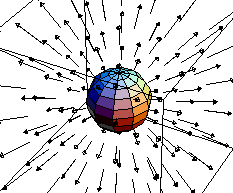
\includegraphics[scale=0.4]{divergencia_0}\caption{{\small Divergencia positiva}}
		\end{center}
	\end{figure}
\end{minipage}
\begin{minipage}{0.7\textwidth}
	\begin{tikzpicture}
		\node[definicion](box){
			\begin{minipage}{0.9\textwidth}
				Sea $\vect{F}:U \subseteq R^n \to R^n,\,\vect{F}\left(\bar{x}\right)=(F_1,F_2,\ldots,F_n)$ un campo diferenciable definido en el abierto $U$ de $R^n$.\\
				
				Se llama \textbf{divergencia} de $\vect{F}$ a:
				\begin{align}
					div(\vect{F})=\frac{\partial F_1}{\partial x_1}+\frac{\partial F_2}{\partial x_2}+\ldots+\frac{\partial F_n}{\partial x_n}
				\end{align}
				Si el campo vectorial $\vect{F}$ representa el flujo de un líquido, entonces la divergencia de $\vect{F}$ representa la expansión o compresión del fluido. Es una medida del \emph{flujo} por unidad de área del líquido a través del punto $p$.
			\end{minipage}};
		\node[fancytitle, right=10pt] at (box.north west) {Divergencia};
		\node[fancytitle, rounded corners] at (box.south) {$\aleph$};
	\end{tikzpicture}
\end{minipage}

\subsection{Teorema de Green}
\begin{minipage}{0.65\textwidth}
	\begin{tikzpicture}
		\node[teorema](box){
			\begin{minipage}{0.9\textwidth}
				\textbf{Hipótesis:}
				\begin{enumerate}
					\item $\vect{F} \in C^1$ en todo punto de $D$ y de $\partial D$
					\item $D$ es una región compacta de $R^2$
					\item $\partial D$ es una curva cerrada, suave a trozos, recorrida en sentido positivo
				\end{enumerate}

				\textbf{Teorema}: Sea $\vect{F}: U \subset R^2 \rightarrow R^2$, $\vect{F}(x,y)=(P,Q)$ un campo de clase $\mathcal{C}^1$ definido en $U$. Sea $D \subset U$ una región plana con su frontera una curva cerrada positivamente orientada (contrario a las agujas del reloj).Entonces:
				\begin{align}
					\oint_{\partial D^{+}}\vect{F} \cdot d\vect{l}=\iint_{D}\left(\frac{\partial Q}{\partial x}-\frac{\partial P}{\partial y}\right)\: dxdy
				\end{align}

				\underbar{Una aplicación}: Si $\vect{F}=(P,Q)$ es tal que $Q^\prime_{x}-P^\prime_{y}=1$, entonces\\
				$\oint_{\partial D^+}\vect{F} \cdot d\vect{s}=\iint_{D}\, dxdy=$ área de $D$.
			\end{minipage}
			};
		\node[fancytitle, right=10pt] at (box.north west) {Teorema de Green};
		\node[fancytitle, rounded corners] at (box.south) {$\aleph$};
	\end{tikzpicture}
\end{minipage}
\begin{minipage}{0.3\textwidth}
	\begin{figure}[H]
		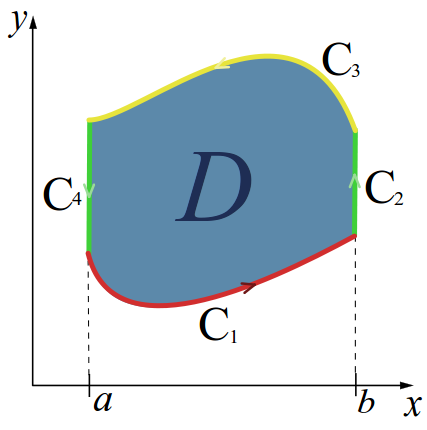
\includegraphics[scale=0.2]{green}
	\end{figure}
\end{minipage}

\subsection{Teorema del rotor (Stokes)}
\begin{minipage}{0.65\textwidth}
	\begin{tikzpicture}
		\node[teorema](box){
			\begin{minipage}{0.9\textwidth}
				\textbf{Hipótesis:}
				\begin{enumerate}
					\item $\vect{F}\in C^1$ en todo punto de $S$ y de $\partial S$
					\item $S$ es una superficie abierta, suave a trozos, simple, parametrizada por una función de clase $C^2$
					\item $\partial S$ es una curva cerrada simple, suave a trozos, y está recorrida en sentido positivo respecto a la superficie
				\end{enumerate}

				\textbf{Teorema}: Sea $S$ una superficie simple orientable, parametrizada por $\phi: D \subset R^3 \to R^3$ de clase $\mathcal{C}^2$, la cual proporciona la orientación de $S$, y sea $\partial S$ su frontera recorrida positivamente. Sea $\vect{F}: U \subseteq R^3 \to R^3$ un campo vectorial de clase $\mathcal{C}^1$ definido en $U$ que contiene a $D$. Entonces:
				\begin{align}
					\oint_{\partial S^{+}}\vect{F} \cdot d\vect{l} & =\iint_{S}\text{rot}(\vect{F}) \cdot d\vect{s}=\iint_{S}\text{rot}\vect{F}(\phi(u,v)) \cdot n_{\phi(u,v)}\: dudv
				\end{align}
				El teorema del rotor es una generalización del teorema de Green. Es importante destacar que para el cálculo de la circulación de una curva $C$ podemos elegir cualquier superficie $S$ que tenga como borde a $C$, y obviamente nos conviene elegir la superficie más \emph{sencilla} posible.\\
				
				\emph{Ejemplo}: Si $C$ es un círculo, $S$ podría ser una circunferencia.
			\end{minipage}
			};
		\node[fancytitle, right=10pt] at (box.north west) {Teorema del rotor (Stokes)};
		\node[fancytitle, rounded corners] at (box.south) {$\aleph$};
	\end{tikzpicture}
\end{minipage}
\begin{minipage}{0.3\textwidth}
	\begin{figure}[H]
		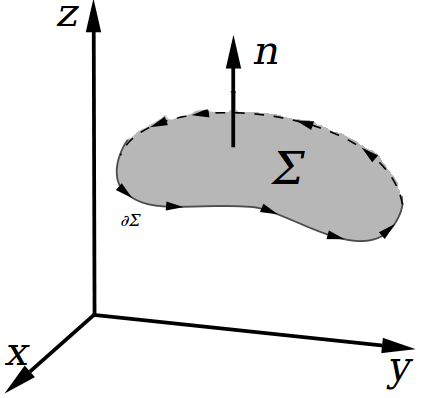
\includegraphics[scale=0.22]{stokes}
	\end{figure}
\end{minipage}

\subsection{Teorema de la divergencia (Gauss)}
\begin{minipage}{0.65\textwidth}
	\begin{tikzpicture}
		\node[teorema](box){
			\begin{minipage}{0.9\textwidth}
				\textbf{Hipótesis:}
				\begin{enumerate}
					\item $\vect{F} \in C^1$ en todo punto de $W$ y de $\partial W$
					\item $W$ un cuerpo compacto de $R^3$
					\item $\partial W$ suave a trozos y orientable, con sus normales hacia afuera
				\end{enumerate}

				\textbf{Teorema}: Sea $W$ un cuerpo de $R^3$ y sea $\partial W$ la frontera de $W$, una superficie orientada con sus vectores normales apuntando hacia el exterior del sólido. Si $\vect{F}: U \subset R^3 \rightarrow R^3$,	$\vect{F}(x,y,z)=(F_1,F_2,F_3)$ es un campo vectorial de clase $\mathcal{C}^1$ definido en el abierto $U$ que contiene a $W$, entonces:
				\begin{align}
					\iint_{\partial W}\vect{F}\cdot d\vect{s}=\iiint_{W}div(\vect{F})\: dxdydz
				\end{align}
				El integrando de la integral triple puede pensarse como la expansión de un fluido. El teorema de la divergencia dice que la expansión total de un fluido que está dentro de un cuerpo $W$ es igual al flujo total del fluido que sale por la frontera del cuerpo $W$.
			\end{minipage}};
		\node[fancytitle, right=10pt] at (box.north west) {Teorema de la divergencia (Gauss)};
		\node[fancytitle, rounded corners] at (box.south) {$\aleph$};
	\end{tikzpicture}
\end{minipage}
\begin{minipage}{0.3\textwidth}
	\begin{figure}[H]
		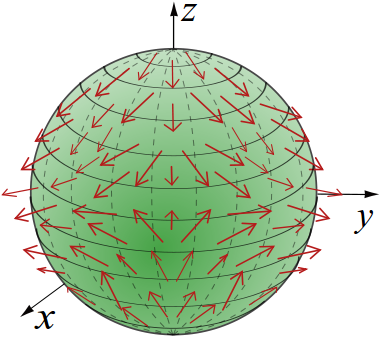
\includegraphics[scale=0.21]{gauss}
	\end{figure}
\end{minipage}

% Bibliografía utilizada en el apunte
\newpage
\newcommand{\bibliographyname}{Bibliografía} % Defino el nombre de la sección de la bibliografía
\addcontentsline{toc}{section}{\bibliographyname} % Agrego la bibliografía en el índice
\renewcommand\refname{\bibliographyname} % Renombro a la bibliografía (por default es 'Referencias')
\begin{thebibliography}{X}
	\bibitem{Marsden} \textsc{Jerrold E. Marsden} y \textsc{Anthony J. Tromba}, \textit{Cálculo Vectorial}, tercera edición, Addison-Wesley Iberoamericana, 1991.
\end{thebibliography}

% Nombres de las personas que han colaborado en la creación del apunte
\colaborador{María Inés Parnisari (maineparnisari@gmail.com)}
\colaborador{Martín Menendez (menendez91@live.com.ar)}
\makeseccioncolaboradores % Crea la seccion de colaboradres

% Incluir el historial de cambios
\revision{26/12/2014}{Versión inicial}
\makehistorial

\end{document}
